\documentclass[footsepline,footinclude=false,oneside,fontsize=11pt,paper=a4,listof=totoc,bibliography=totoc]{scrbook} % one-sided

\setkomafont{disposition}{\normalfont\bfseries} % use serif font for headings
%\linespread{1.05} % adjust line spread for mathpazo font

\usepackage{nameref}
\usepackage[utf8]{inputenc}
\usepackage[T1]{fontenc}
%\usepackage[sc]{mathpazo}
\usepackage[american]{babel}
\usepackage[autostyle]{csquotes}
\usepackage[%
backend=biber,
url=false,
style=numeric,
maxnames=4,
minnames=3,
maxbibnames=99,
giveninits,
uniquename=init]{biblatex}
\bibliography{bachelor_thesis}
% \addbibresource{bachelor_thesis.bib}
\usepackage{graphicx}
\usepackage{scrhack} % necessary for listings package
\usepackage{listings}
\usepackage{lstautogobble}
\usepackage{tikz}
\usetikzlibrary {positioning}
\usetikzlibrary{shapes,arrows}
\usetikzlibrary{automata, arrows.meta, positioning}
\usepackage{pgf}
\usepackage{pgfplots}
\pgfplotsset{compat=1.18}
\usepackage{pgfplotstable}
\usepackage{booktabs}
\usepackage{minibox}
\usepackage{longtable}
\usepackage{multirow}
\usepackage[final]{microtype}
\usepackage[singlelinecheck=false, figurename=Fig., aboveskip=7pt, belowskip=0pt]{caption}
\setcapindent{10pt}

\usepackage{prettyref}
\usepackage{titleref}
\usepackage[hidelinks, pdfpagelabels, pdfstartview = FitH, bookmarksopen = true, bookmarksnumbered = true,
plainpages = false, hypertexnames = false, citecolor = black] {hyperref}
\usepackage[toc,nonumberlist,acronym]{glossaries} % TODO: remove if glossary not needed
\usepackage{acronym}

\usepackage{afterpage} %for using \afterpage{\clearpage} (don't push images to the end of a chapter)
\usepackage{picins} %provides precise control over the placement of inline graphics
\usepackage{setspace}
%\usepackage{titlesec}
\usepackage{dsfont} %math symbols
\usepackage{tabularx}
\usepackage{subcaption}
\usepackage{picture}

\usepackage{enumitem} %resume counting from previous enumerate block
\usepackage{amsmath,amssymb}
\usepackage{listings} %for listing source code
\usepackage{color}
\usepackage{algpseudocode} %for listing pseudocode
\usepackage{algorithm} %wrap algpseudocode and enrich with label etc.
%\usepackage{float} % for [H] after floats
%\usepackage{floatflt}
\usepackage{verbatim}
\usepackage{xparse}
\usepackage{fancyvrb}
\usepackage{fvextra}
\usetikzlibrary{arrows,automata}
\usetikzlibrary{positioning}
\usetikzlibrary{calc}

%\usepackage{subfig}

\DeclareCaptionLabelFormat{custom}
{%
	#1 (#2)
}
% Separator style
\DeclareCaptionLabelSeparator{custom}{}
% Caption format    
\DeclareCaptionFormat{custom}
{%
	\small#1#2 #3
}
\captionsetup
{
	format=custom,%
	labelformat=custom,%
	labelsep=custom
}

\newcommand{\todo}[1]{\textbf{\color{red} #1}}

\newcommand{\thesistitle}{Inferring String Properties from Code Property Graphs}
\newcommand{\name}{Severin Schmidmeier}
\newcommand{\submission}{15.03.2023}

\newrefformat{fig}{Figure~\ref{#1}}	%link to a figure
\newrefformat{chapter}{Chapter~\ref{#1}}	%link to a chapter
\newrefformat{sec}{Section~\ref{#1}}	%link to a section
\newrefformat{tab}{Table~\ref{#1}}	%link to a table
\newrefformat{lst}{Listing~\ref{#1}}	%link to a listing

\newtheorem{Def}{Definition}[chapter]

\makeindex
\frenchspacing
\sloppy

\lstset{language=Java,
		basicstyle=\ttfamily,
	tabsize=4,}

 
\begin{acronym}
	\acro{ast}[AST]{abstract syntax tree}
	\acro{cfg}[CFG]{context-free grammar}
	\acro{cfl}[CFL]{context-free language}
	\acro{cpg}[CPG]{Code Property Graph}
	\acro{dag}[DAG]{directed acyclic graph}
	\acro{dfa}[DFA]{deterministic finite automaton}
	\acro{dfg}[DFG]{data flow graph}
	\acro{gnfa}[GNFA]{generalized nondeterministic finite automaton}
	\acro{mlfa}[MLFA]{multi-level automaton}
	\acro{nfa}[NFA]{nondeterministic finite automaton}
	\acro{pql}[PQL]{Process Query Language}
	\acro{scc}[SCC]{strongly connected component}
	\acro{srg}[SRG]{strongly regular grammar}
\end{acronym}

%\pagestyle{headings}

%\textwidth16cm
%\textheight22cm

%\topmargin0cm
%\oddsidemargin0cm
%\evensidemargin0cm

% This is tumlogo.tex
%
% Neues TUM-Logo in TeX
%   by G. Teege, 19.10.89
% Benutzung:
%   Am Anfang des Dokuments (TeX oder LaTeX):
%     \input tumlogo
%   Dann beliebig oft:
%     \TUM{<breite>}
%   bzw.
%     \oTUM{<breite>}
%   \TUM setzt das Logo mit der Breite <breite> und der entsprechenden Hoehe.
%   <breite> muss eine <dimen> sein. \oTUM erzeugt eine "outline"-Version
%   des Logos, d.h. weiss mit schwarzem Rand. Bei \TUM ist es ganz schwarz.
%   \oTUM entspricht damit der offiziellen Version des Logos.
%   Das Logo kann wie ein einzelnes Zeichen verwendet werden.
%   Beispiel:
%     Dies ist das TUM-Logo: \oTUM{1cm}.
%
\def\TUM#1{%
\dimen1=#1\dimen1=.1143\dimen1%
\dimen2=#1\dimen2=.419\dimen2%
\dimen3=#1\dimen3=.0857\dimen3%
\dimen4=\dimen1\advance\dimen4 by\dimen2%
\setbox0=\vbox{\hrule width\dimen3 height\dimen1 depth0pt\vskip\dimen2}%
\setbox1=\vbox{\hrule width\dimen1 height\dimen4 depth0pt}%
\setbox2=\vbox{\hrule width\dimen3 height\dimen1 depth0pt}%
\setbox3=\hbox{\copy0\copy1\copy0\copy1\box2\copy1\copy0\copy1\box0\box1}%
\leavevmode\vbox{\box3}}
%
\def\oTUM#1{%
\dimen1=#1\dimen1=.1143\dimen1%
\dimen2=#1\dimen2=.419\dimen2%
\dimen3=#1\dimen3=.0857\dimen3%
\dimen0=#1\dimen0=.018\dimen0%
\dimen4=\dimen1\advance\dimen4 by-\dimen0%
\setbox1=\vbox{\hrule width\dimen0 height\dimen4 depth0pt}%
\advance\dimen4 by\dimen2%
\setbox8=\vbox{\hrule width\dimen0 height\dimen4 depth0pt}%
\advance\dimen4 by-\dimen2\advance\dimen4 by-\dimen0%
\setbox4=\vbox{\hrule width\dimen4 height\dimen0 depth0pt}%
\advance\dimen4 by\dimen1\advance\dimen4 by\dimen3%
\setbox6=\vbox{\hrule width\dimen4 height\dimen0 depth0pt}%
\advance\dimen4 by\dimen3\advance\dimen4 by\dimen0%
\setbox9=\vbox{\hrule width\dimen4 height\dimen0 depth0pt}%
\advance\dimen4 by\dimen1%
\setbox7=\vbox{\hrule width\dimen4 height\dimen0 depth0pt}%
\dimen4=\dimen3%
\setbox5=\vbox{\hrule width\dimen4 height\dimen0 depth0pt}%
\advance\dimen4 by-\dimen0%
\setbox2=\vbox{\hrule width\dimen4 height\dimen0 depth0pt}%
\dimen4=\dimen2\advance\dimen4 by\dimen0%
\setbox3=\vbox{\hrule width\dimen0 height\dimen4 depth0pt}%
\setbox0=\vbox{\hbox{\box9\lower\dimen2\copy3\lower\dimen2\copy5%
\lower\dimen2\copy3\box7}\kern-\dimen2\nointerlineskip%
\hbox{\raise\dimen2\box1\raise\dimen2\box2\copy3\copy4\copy3%
\raise\dimen2\copy5\copy3\box6\copy3\raise\dimen2\copy5\copy3\copy4\copy3%
\raise\dimen2\box5\box3\box4\box8}}%
\leavevmode\box0}
% End of tumlogo.tex



\begin{document}

\nocite{*} %include uncited references in bibliography
\hoffset=5mm
\thispagestyle{empty}

\begin{center}
	\bigskip \bigskip \bigskip
	\oTUM{5.0cm} \\
	\vspace*{0.8cm}
	{\huge SCHOOL OF COMPUTATION, INFORMATION AND TECHNOLOGY --- INFORMATICS} \\
	\bigskip \bigskip
	{\Large TECHNISCHE UNIVERSIT\"AT M\"UNCHEN} \\
	\bigskip \bigskip \bigskip \bigskip \bigskip
	{\Large Bachelor's Thesis in Informatics} \\
	\bigskip \bigskip \bigskip \bigskip \bigskip
	{\LARGE \textbf \thesistitle} \\
	\bigskip \bigskip \bigskip \bigskip
	{\Large \name} \\    
	\bigskip\bigskip
	\begin{figure}[htbp]
	\centering 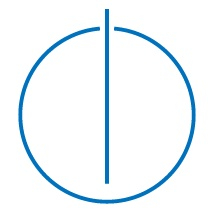
\includegraphics[width=3cm]{logos/infologo.jpg}
	\end{figure}
	\bigskip 
\end{center}

\vfill

\newpage
\hoffset=5mm
\thispagestyle{empty}

\begin{center}
	\bigskip \bigskip \bigskip 
	\oTUM{5.0cm} \\
	\vspace*{0.8cm}
	{\huge SCHOOL OF COMPUTATION, INFORMATION AND TECHNOLOGY --- INFORMATICS} \\
	\bigskip \bigskip 
	{\Large TECHNISCHE UNIVERSIT\"AT M\"UNCHEN} \\
	\bigskip \bigskip \bigskip \bigskip
	{\Large Bachelor's Thesis in Informatics} \\
	\bigskip \bigskip \bigskip \bigskip
	{\Large \thesistitle} \\   
	\bigskip \bigskip
	{\Large Herleitung von Eigenschaften von Strings aus Code Property Graphen} \\
	\bigskip
\vfill

\begin{tabular}{ll}
{\large Author:} & {\large \name} \\\\
{\large Supervisor:} & {\large Prof. Dr. Claudia Eckert} \\\\
{\large Advisor(s):} & {\large Alexander K\"uchler, Florian Wendland} \\\\
{\large Submission:} & {\large \submission}
\end{tabular}\bigskip

\begin{figure}[htbp]
\centering 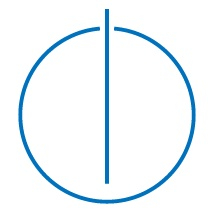
\includegraphics[width=3cm]{logos/infologo.jpg}
\end{figure}
\bigskip
\end{center}

\newpage	
\thispagestyle{empty}
\hoffset=0mm
\vspace*{\fill}
\noindent I confirm that this bachelor's thesis is my own work and I have documented all sources and material used.\\\\
Ich versichere, dass ich diese Bachelorarbeit selbstst\"andig verfasst und nur die angegebenen Quellen und Hilfsmittel verwendet habe.\\\\\\
M\"unchen, \submission\\\\\\\\\\\\
\noindent \textit{(\name)}

\newpage
\setcounter{page}{1}
\pagenumbering{roman}
\begin{spacing}{1.2}
\hoffset=0mm
\input acknowledgements

\input abstract
\end{spacing}

%\setcounter{tocdepth}{3}
%\setcounter{secnumdepth}{3}
%\fboxsep 0mm

\tableofcontents

\newpage
\setlength{\baselineskip}{3ex}
\setcounter{page}{1}
\pagenumbering{arabic}

\begin{spacing}{1.15}

\chapter{Introduction}
\label{chapter:introduction}

\begin{comment}
	Your introduction goes here
	\begin{itemize}
		\item Generic description of the broad field of research
		\item Current state of research
		\item What's the gap that you're trying to fill?
		\item Short motivation
		\item Summary of the most important results
		\item Your contribution
		\item Structure of the thesis
	\end{itemize}
	
	1-2.5 pages
	
	This text is not too detailed. Start quite high-level, then narrow down until
	you reach your topic. After the introduction, the reader must want to read the
	rest of your thesis and understand the relevance. However, it doesn't have to
	be super technical.
\end{comment}

\section{Motivation}

The increasing reliance on software applications in various aspects of modern life has led to a growing concern for the security of these applications. Among the many security threats that can affect software, injection vulnerabilities are among the most dangerous and prevalent. According to the Open Web Application Security Project (OWASP), injection attacks, which include SQL injection, LDAP injection, and command injection, are consistently listed as one of the top ten web application security risks\footnote{https://owasp.org/Top10}.

Injection vulnerabilities occur when an attacker is able to insert malicious code or input into an application, often through input fields that accept user input such as search boxes or login forms. This can result in the attacker gaining unauthorized access to sensitive data, executing arbitrary code, or even taking control of the entire system.

To prevent injection vulnerabilities, developers can use a variety of tools and techniques, including static analysis tools for string values. These tools analyze the source code of an application to identify potential vulnerabilities, including injection vulnerabilities. Static analysis tools are particularly useful because they can detect vulnerabilities that may not be apparent during testing or manual code review.

In order to detect injection vulnerabilities, such tools can try to analyze the possible values a string that is passed as a query to e.g. a database can take on.

From these inferred properties, a tool can then assess, whether the analyzed program contains any potential injection vulnerabilities and warn the programmer.

\section{Contribution}

In this thesis, we extend a \acf{cpg} implementation, which is used by the static analysis tool Codyze\footnote{https://www.codyze.io/}, to increase its capabilities in analyzing string values. We adapt a theoretical approach \cite{brics}, which creates regular languages describing the values of a string, to the present \ac{cpg} implementation. We combine this approach with other techniques \cite{delgado}\cite{nederhof} to improve the results and provide them as regular expressions to users. We also provide a working proof of concept implementation covering a subset of the Java standard library.

After providing some theoretical background in Chapter \ref{chapter:Background}, we describe the different steps of our approach in Chapter \ref{chapter:Approach}.
In Chapter \ref{chapter:Evaluation}, we then evaluate the results and benchmark our implementation. There, we also highlight some limitations of our approach and include ideas for future continuation and improvement of the presented design. We present some related work in Chapter \ref{chapter:RelatedWork} before concluding the outcome of this thesis in Chapter \ref{chapter:Conclusion}.


\chapter{Problem Description}
\label{chapter:ProblemDescription}

The introduction is a bit like a teaser. Here, you dig more into details, also
technical ones. After this chapter, the reader must understand why you do this
work, why it's important, what makes it difficult and what you want to achieve.

\begin{itemize}
\item What's the problem that you're trying to solve?
\item What is your goal?
\item What is/are the research question(s)?
\item What are special problems?
\end{itemize}

Probably 1-3 pages


\chapter{Background}
\label{chapter:Background}
\begin{comment}
What is the knowledge a undergrad student needs so that he/she can understand
your thesis? You can assume some familiarity with the very broad topic. E.g. if
you write a thesis in the area of software analysis, you do not have to explain
static/dynamic analysis as such (this is boring!). If you're a crypto guy, don't
explain AES in detail unless you try to break it in your thesis. If I stumble
across a word/term in your thesis and don't understand it, this is where I would
look it up (or on google).

Probably approx. 3-10 pages
\end{comment}

\section{Preliminaries}

\subsection{Formal Grammars}

A formal grammar consists of a set of nonterminal symbols $N$, an alphabet $\Sigma$ of terminal symbols, a set of production rules $(\Sigma \cup N)^*N(\Sigma \cup N)^* \rightarrow (\Sigma \cup N)^*$, also called just "productions" and a start symbol.

In examples of grammars, we use capital letters for nonterminals and lower case letters for terminals. We also don't specify the start symbol explicitly, but rather the nonterminal on the left hand side of the first production is considered to be the start symbol.

\acfp{cfg} are grammars, where the left hand side of all productions consists of a single nonterminal.
Regular grammars are \acp{cfg}, where the right hand side of each production consists either of a single terminal $a \in \Sigma$ or of exactly one nonterminal and one terminal. Additionally, the nonterminals on the right hand side are either always the first symbol or always the last symbol on the right hand side. A grammar containing both the productions $A \rightarrow aB$ and $B \rightarrow Ab$ with $A, B \in N \land a, b \in \Sigma$ therefore is not regular, as the nonterminal is the last symbol in the first production but the first symbol in the latter.

\subsection{Automata}

A \acf{dfa} consists of a set of states $Q$, an alphabet of input symbols $\Sigma$, a transition function $\delta: Q \times \Sigma \rightarrow Q$, an initial state $q_0 \in Q$ and a set $F \subseteq Q$ of accepting states.
For a \acf{nfa}, from a given state multiple states can be reached with the same input, so the transition function is  $\delta: Q \times \Sigma \rightarrow 2^Q$, where $2^Q$ denotes the power set of $Q$.

We represent automata as graphs, where each state is a node and the transition function is represented by edges labeled with elements of $\Sigma$. The start state is marked with an incoming arrow and the accepting states are marked with double circles.
An edge in this graph, henceforth also called transition, is denoted as $(q_1, a, q_2)$, where $q_1 \in Q$ is the origin state, $a \in \Sigma$ is the label and $q_2 \in Q$ is the target state of the edge.

\section{Strongly Regular Grammars}\label{sec:background:srg}

$\mathcal{R}$ is the equivalence relation defined on the set of nonterminals $N$ of some grammar:

\begin{align}
	A \mathcal{R} B \Leftrightarrow (\exists \alpha, \beta \in V^* : A \xrightarrow{*} \alpha B \beta) \land (\exists \alpha, \beta \in V^* : B \xrightarrow{*} \alpha A \beta) 
\end{align}

Here $V$ is $\Sigma \cup N$, so the set of all symbols, terminal and nonterminal. $\xrightarrow{*}$ is the reflexive and transitive closure of the production relation $\rightarrow$ defined by the set of productions in the grammar. $A \xrightarrow{*} \alpha B \beta$ means, that there exists a sequence of productions starting at the symbol $A$ to produce a set of symbols that contain $B$. Therefore $\mathcal{R}$ groups all nonterminals into disjoint equivalence classes, where each nonterminal in a class can be produced by each other nonterminal in the class. Those nonterminals are called mutually recursive.

A grammar is strongly regular if the production rules in each such equivalence class are either all right-linear or left-linear.

A production rule is right-linear if it is of the form $A \rightarrow w \alpha$, where $w$ is a sequence of terminal symbols and $\alpha$ is empty or a single nonterminal symbol. Left-linear productions are defined accordingly but the nonterminal is on the left side of the production result.


\section{Code Property Graph}
The library\footnote{https://github.com/Fraunhofer-AISEC/cpg} we extend in this thesis extracts a \ac{cpg} out of source code of a set of different programming languages.

This graph is used as a backend in the static analysis tool Codyze\footnote{https://www.codyze.io}.

The \ac{cpg} is a directed multi graph, where the nodes represent syntactic elements like simple expressions or function declarations and the edges represent the relations between those elements. The nodes and edges have a list of key - value pairs called properties which contain general information for the element. For example, a Node representing a statement in a source file contains the location of the underlying code and an edge representing evaluation order may contain whether the target statement is unreachable. The graph is initially created by language frontends, which create partially connected \acp{ast}, which are then enriched by additional information like the mentioned evaluation order by multiple passes \cite{cpg}.

Users of the library can extend this functionality by adding additional passes, which is how we implement the hotspot collection in this thesis.

% eher motivation
% The \ac{cpg} makes it possible to find weaknesses and vulnerabilities in source code of different programming languages. Since strings are part of most software, making detailed information about them available for analysis could improve this application of the \ac{cpg}.

While the \ac{cpg} contains many different types of edges, the most relevant edge type for this thesis are data flow edges, which represent the data flow between different expressions.

\begin{lstlisting}[label={lst:stringCreation}, caption={Example code}, captionpos=b]
	String s = "xyz";
	System.out.println(s);
\end{lstlisting}

Consider the short code example in listing \ref{lst:stringCreation}. Here, among others, the following nodes are part of the \ac{cpg}:

\begin{itemize}
	\item \lstinline|Literal|, representing the string literal \lstinline{"xyz"}
	\item \lstinline|VariableDeclaration|, representing the declaration and initialization of the variable \lstinline|s|
	\item \lstinline|DeclaredReferenceExpression|, representing the reference to the variable \lstinline|s| in line 2.
\end{itemize}

In this example, the data flows from the \lstinline|Literal| node to the \lstinline|VariableDeclaration| and from there to the \lstinline|DeclaredReferenceExpression|.

The nodes connected by those egdes effectively form a subgraph of the \ac{cpg}, the \ac{dfg}, from which we then extract the information on string values.

% TODO mention definition for DFG in CPG repo




\chapter{Approach and Implementation}
\label{chapter:Approach}


We first provide a general overview of our approach and describe which steps are needed for the transformation from \ac{dfg} to regular expression. Subsequently, we provide a detailed description of each step.


\section{General Approach}

The general approach for our implementation is adapted from the one described by Christensen et al. \cite{brics}. Conceptually, we first create a \acf{cfg} from the \ac{dfg} in the process described in Section \ref{sec:grammarCreation}.
The created \ac{cfg} is then approximated to a \acf{srg} using the Character Set Approximation described in Section \ref{sec:charsetApprox} and the Mohri-Nederhof algorithm described in Section \ref{sec:mohriNederhofApprox}. We then transform this \ac{srg} into a \acf{nfa} using Nederhof's algorithm described in Section \ref{sec:nederhofAlgorithm}. Finally, we describe how to create a regular expression from this automaton using the state elimination strategy in Section \ref{sec:nfa2regex}. The following diagram visualizes this process and the different steps from a graph to different types of formal grammars to a regular expression.


\tikzstyle{grammar} = [
	rectangle, 
	draw, 
	fill=gray!20, 
	text width=5em, 
	text centered, 
	rounded corners, 
	minimum size=2cm,
	thick
	]
\tikzstyle{automaton} = [
	circle, 
	draw, 
	fill=blue!20, 
	text width=5em, 
	text centered,
	minimum size=2cm,
	thick
]
\tikzstyle{graph} = [
	ellipse, 
	draw, 
	fill=orange!20, 
	text width=5em, 
	text centered,
	minimum height=1.5cm,
	minimum width=1cm,
	text width=1.5cm,
	align=center,
	thick
	]
\tikzstyle{result} = [
	rectangle, 
	draw, 
	fill=green!20, 
	text width=5em, 
	text centered, 
	minimum size=2cm,
	thick
	]
\tikzstyle{line} = [draw, -latex', very thick]
\begin{figure}[H]
	\centering
\begin{tikzpicture}[node distance=2cm and 2.5cm, auto]
	    \node [graph] (DFG) {\ac{dfg}};
	    \node [grammar, right=of DFG] (CFG) {\ac{cfg}};	    
	    \node [automaton, below= of CFG] (nfa) {\ac{nfa}};
	    \node [result, left=of nfa] (regex) {regular expression};
 	    \node [grammar, right=of nfa, xshift=1.5cm] (REG) {\ac{srg}};
	    
	    \path [line] (DFG) -> node[above, align=center] {grammar\\creation} (CFG);
	    \path [line] (CFG) -| coordinate (midpoint) (REG);
	    \path [line] (CFG) -> node [above, midway] {charset approximation} (midpoint);
 	    \path [line] (midpoint) -> node [left, midway, align=center] {Mohri-Nederhof\\approximation} (REG);
	    \path [line] (REG) -> node[above, align=center] {Nederhof's\\algorithm} (nfa);
	    \path [line] (nfa) -> node[above, align=center] {state\\elimination} (regex);
\end{tikzpicture}
\caption{The general approach for obtaining regular expressions}
\label{fig:approach}
\end{figure}


\section{Grammar Creation}\label{sec:grammarCreation}
To create the grammar for a given \ac{cpg} node, we traverse the \ac{dfg} backwards, starting at the given node. 
% The starting node can be one of the hotspot nodes collected by the aforementioned \lstinline|Pass|, but in general the grammar creation is independent of the hotspot collection.
For each visited node, we add a \lstinline|Nonterminal| and the fitting productions to our grammar. 

The different types of productions we use can be seen in Table \ref{tab:productions}, where \texttt{<terminal>} represents a terminal symbol containing a regular expression that describes a string value and \enquote{$op$} is a placeholder for a string operation that is applied to some arguments.

\begin{table}[H]
	\centering
	\begin{tabular}{ccc}
		\toprule
		\thead{\textbf{Name}} & \thead{\textbf{Production}} & \thead{\textbf{Usage}} \\
		\midrule
		\makecell{\lstinline|UnitProduction|} & \makecell{$X \rightarrow Y$} & \makecell{references between nodes} \\
				\midrule
		\makecell{\lstinline|ConcatProduction|} & \makecell{ $X \rightarrow Y\ Z$} & \makecell{concatenation of two nodes} \\
				\midrule
		\makecell{\lstinline|TerminalProduction|} & \makecell{$X \rightarrow \texttt{<terminal>}$} & \makecell{literal string values and\\other terminal symbols} \\
				\midrule
		\makecell{\lstinline|OperationProduction|} & \makecell{$X \rightarrow op(Y)$} & \makecell{operations on strings} \\
		\bottomrule
	\end{tabular}
	\caption{Utilized production types}
	\label{tab:productions}
\end{table}

Consider the code example in Listing \ref{lst:grammar_example} for the following explanations of the different productions.

\begin{lstlisting}[label={lst:grammar_example}, caption={Grammar creation example code},escapeinside={(*}{*)}, numbers=right, captionpos=b]
	String s(*\textcolor{red}{$^1$}*) = " foo";
	s(*\textcolor{red}{$^2$}*) = s(*\textcolor{red}{$^3$}*) + "bar";
	s(*\textcolor{red}{$^4$}*) = s(*\textcolor{red}{$^5$}*).trim();
\end{lstlisting}

\lstinline|UnitProduction|s mostly represent references between nodes where the underlying string is not changed. In Listing \ref{lst:grammar_example}, this would be the case for the reference from \lstinline|s|$^3$ to the variable declaration in line 1. 

\lstinline|ConcatProduction|s are created for \lstinline|BinaryOperator| nodes that represent a string concatenation using the \lstinline|+| operator. For the example in Listing \ref{lst:grammar_example}. the nonterminal corresponding to the \lstinline|BinaryOperator| node for the \lstinline|+| in line 2 would have a \lstinline|ConcatProduction| with the right hand side nonterminals corresponding to the nodes for \lstinline|s|$^3$ and the string literal respectively.

\lstinline|TerminalProduction|s point to a \lstinline|Terminal| that represents a fixed regular expression.
For example, for the \lstinline|Literal| \ac{cpg} node representing the \lstinline|"bar"| string literal, the corresponding nonterminal has a \lstinline|TerminalProduction| where the \lstinline|Terminal| contains a regular expression that matches only the string \enquote{bar}. \lstinline|TerminalProduction|s also occur at \ac{cpg} nodes without incoming \ac{dfg} edges where the value is not known. Those nodes could represent any string value, and therefore, the corresponding \lstinline|Terminal| contains the regular expression \lstinline|.*|, matching all strings.

\lstinline|OperationProduction|s represent function calls or other operators. The \ac{cpg} for Listing \ref{lst:grammar_example} contains a \lstinline|CallExpression| representing the function call to the library function \lstinline|trim|. We create a \lstinline|Trim| object representing this operation and the \lstinline|OperationProduction| $X \rightarrow trim(Y)$, where $X$ is the nonterminal corresponding to the node representing \lstinline|s|$^4$ and $Y$ to the one representing \lstinline|s|$^5$. 
All operation objects like \lstinline|Trim| also contain information about possible arguments and implement a character set transformation and an automaton transformation. These transformations describe the effect of the operation on the set of characters making up the words the operation is applied on or automata accepting those words respectively.
Examples and how these transformations are used for the approximation are described in Section \ref{sec:approximation}.
This language agnostic representation of string operations allows developers of the \ac{cpg} library to add support for functions and operators in other languages with different semantics compared to the corresponding Java functions, without needing to change the grammar approximation. For example, for the Python expression \lstinline[language=Python]|"abc" * 5|, the \lstinline|*| operator can be represented using a generic \lstinline|Repeat| operation object. For all further steps it is not relevant whether this repeat operation is created from the mentioned Python operator \lstinline[language=Python]|s * n| or from the corresponding Java function \lstinline|s.repeat(n)|. 


\subsubsection{Improvements}

Unlike Christensen et al. \cite{brics}, we do not consider the total \ac{dfg} when extracting the grammar. They parse the whole graph into a grammar describing all nodes, while we create the grammar starting from a single node and ignore all parts of the graph not connected via \ac{dfg} edges to this node.

Since the majority of a large program is often not relevant for a specific node, this reduces the amount of nodes we need to handle during analysis. Consequently, this reduces the size of the resulting grammar, therefore leading to performance improvements.

Additionally, we can traverse the \ac{dfg} conditionally, stopping at nodes representing numbers. If the traversal reaches such a node, we use an existing analysis that tries to compute the precise value.
For example, for an integer created by the usual arithmetic operations, this analysis can obtain the resulting value.
In this case, we can add a \lstinline|TerminalProduction| with the \lstinline|Terminal| representing the value literal and otherwise, if the value is not known, the \lstinline|Terminal| contains a regular expression matching all numbers of the present type, e.g. \lstinline{"0|(-?[1-9][0-9]*)"} for integrals.
	

\section{Regular Approximation}\label{sec:approximation}

To transform the created grammar into a regular expression, we need to approximate the \ac{cfg} we obtained like described in the previous section. Since basic regular expressions accept regular languages, the result of this approximation has to be a type of grammar that produces only regular languages to allow direct conversion to regular expressions without losing information. Using the two different approximation steps described in the following section, the \ac{cfg} is approximated into a \acl{srg}.

\subsection{Character Set Approximation}\label{sec:charsetApprox}
To use the Mohri-Nederhof approximation algorithm described in Section \ref{sec:mohriNederhofApprox}, we first need to eliminate all cycles in our grammar that contain operation productions \cite{mohri_nederhof}.

First, we view the grammar as a graph in which each symbol of the grammar corresponds to one graph node and for each production there are edges from the nonterminal on the left hand side to all symbols on the right hand side. 
For two nonterminals $A$ and $B$, there is an edge from the node corresponding to $A$ to the one corresponding to $B$ if and only if there exists a production of form $A \rightarrow \alpha B \beta$ with $\alpha$ and $\beta$ sequences of arbitrary symbols.
This graph allows us to group terminals that are reachable from each other by finding the \acp{scc} of the graph.

All nonterminals are assigned a character set, containing all characters that make up the words in the language of the corresponding nonterminal.

\begin{figure}[!h]
	\begin{align*}
		&S \rightarrow replace[c, x](A)\\
		&A \rightarrow BC | CB\\
		&B \rightarrow "ba"\\
		&C \rightarrow "ca"
	\end{align*}
	\caption{Example grammar}
	\label{fig:charset:grammar}
\end{figure}

We assign a character set to each nonterminal $N$ using a fixed-point iteration inside the graph component of $N$ that constructs a character set $C(N)$ for $N$ from the character sets of the nonterminals on the right hand side of $N$'s productions.

For productions with terminals on the right hand side, the character set is just the set of all characters occurring in the terminal. To account for the terminals that are regular expressions and therefore may include meta characters, which should not be included in the character set, we create the character set when we construct the regular expression. Consider, for example, the regular expression representing integers mentioned above. There, the corresponding character set contains all digit characters and the minus sign.
For concatenation productions like $A \rightarrow BC$ in the example above, we take the union of the character sets of the two nonterminals on the right hand side.

Considering the example grammar in Figure \ref{fig:charset:grammar}, $B$ represents the word $ba$ and and $C$ represents $ca$, therefore the corresponding sets of characters are  $\{\text{'a', 'b'}\}$ and  $\{\text{'a', 'c'}\}$ respectively. The words that can be generated from $A$ are combinations of $B$ and $C$ and therefore always contain all characters in the character sets of $B$ and $C$. Thus, the character set for $A$ is $\{\text{'a', 'b'}\} \cup \{\text{'a', 'c'}\} = \{\text{'a', 'b', 'c'}\}$.

Each operation defines a character set transformation - a function $T_{op} : 2^\Sigma \rightarrow 2^\Sigma$ - that approximates how the application of the given operation changes the character set. Here, $\Sigma$ represents the set of all possible characters.
For example the character set transformation for a \lstinline|replace| operation, where a known character \lstinline|o| is replaced by a known character \lstinline|n| has the character set transformation described in Formula \ref{math:replace:known}.

\begin{align}
	\centering
	T_{replace[o, n]}(S) = 
	\begin{cases}
		(S \setminus \{o\}) \cup \{n\}, & \text{if } o \in S\\
		S, & \text{if } o \notin S
	\end{cases}
	\label{math:replace:known}
\end{align}

In comparison, for a \lstinline|replace| operation, where the newly inserted character is not known, the transformation is defined as shown in Formula \ref{math:replace:unknown}. Here, if the replaced character is contained in $S$, the set is transformed to $\Sigma$, since the newly inserted character could be any element of $\Sigma$.

\begin{align}
	\centering
	T_{replace[o, ?]}(S) = 
	\begin{cases}
		\Sigma & \text{if } o \in S\\
		S, & \text{if } o \notin S
	\end{cases}
	\label{math:replace:unknown}
\end{align}

These approximations are used in the fixed-point computation to assign character sets.
As mentioned above, in the example in Figure \ref{fig:charset:grammar} the character set for $A$ is $\{\text{'a', 'b', 'c'}\}$. To obtain the character set of $S$, we apply the transformation defined by the $replace[c,x]$ operation to the character set of $A$, which gives us $(\{\text{'a', 'b', 'c'}\} \setminus \{\text{'c'}\}) \cup \{\text{'x'}\} = \{\text{'a', 'b', 'x'}\}$ as the character set of $S$.

To determine the \acp{scc}, we use Tarjan's algorithm \cite{tarjan}.
The \acp{scc} of a graph form a \ac{dag}, because if the graph of \acp{scc} would contain a cycle, all contained components would be strongly connected and therefore joined into one component. This \ac{dag} implies that there exists a topological ordering of the \acp{scc} \cite{mit_algorithms}.
Tarjan's algorithm topologically sorts the returned components in reverse order as a byproduct, which is necessary for the fixed-point iteration to terminate.
During the computation, for a given nonterminal $N$, its charset is updated using the character sets of its successors. The reverse topological ordering of the components ensures that the first handled component is the root in the graph formed by the \acp{scc}, while leafs in this graph are handled last. This ensures that the successors of each nonterminal are either in the same component or in a component that has already been handled earlier.

To break up the cycles containing operation productions, we replace one operation production $X \rightarrow op(Y)$ in each cycle with a production $X \rightarrow r$, where $r$ is the regular expression that matches the language $C(X)^*$. Here, $C(X)$ again denotes the character set we assigned to the nonterminal $X$.

To find the cycles in the grammar, we check for each nonterminal $A$ in a given component $M$, whether it has an operation production, and if yes, whether one of the nonterminals on its right-hand side is also part of $M$. If this is the case, by definition of \acp{scc}, $A$ is reachable from this nonterminal and therefore the operation production is part of a cycle.

\subsubsection{Character Set Implementation}

In real world applications, the occurring character sets usually either contain only a few characters, for example the alphanumericals in a string literal, or almost all characters, for example when a single character is removed from an unknown variable represented by $\Sigma$.

We also need to efficiently convert both of these types of sets into short regular expressions to keep the results human-readable. A naive implementation like joining all contained characters using the regular expression choice operator would lead to extremely long expressions for very large sets.

To solve this problem and easily represent these two extremes, we have two different implementations, both conforming to a common \lstinline|CharSet| interface that requires the common set functions \lstinline|union|, \lstinline|intersect|, functionality for adding and removing characters and membership checks.

The first, \lstinline|SetCharSet|, is mostly a simple wrapper around a \lstinline|Set<Char>| containing the characters.
The second, \lstinline|SigmaCharSet|, is used to easily represent sets like $\Sigma \setminus \{a, b, c\}$ by storing a \lstinline|Set<Char>| containing the characters $not$ contained in the set, while all other characters are assumed to be members.

The behavior of the the set operations \lstinline|union| and \lstinline|intersect| can be described using the operations defined in Figure \ref{fig:setops}.

\begin{figure}
\noindent
\begin{alignat*}{3}
	& \text{\lstinline|SigmaCharSet union SigmaCharSet| } && \hat{=}\ (\Sigma \setminus A) \cup (\Sigma \setminus B) & &= \Sigma \setminus (A \cap B) \\
	& \text{\lstinline|SigmaCharSet union SetCharSet| } && \hat{=}\ (\Sigma \setminus A) \cup S & &= \Sigma \setminus (A \setminus S) \\
	& \text{\lstinline|SetCharSet union SetCharSet| } && \hat{=}\ & &\phantom{{}={}} S_1 \cup S_2 \\
	& \text{\lstinline|SigmaCharSet intersect SigmaCharSet| } && \hat{=}\ (\Sigma \setminus A) \cap (\Sigma \setminus B) & &= \Sigma \setminus (A \cup B) \\
	& \text{\lstinline|SigmaCharSet intersect SetCharSet| } && \hat{=}\ (\Sigma \setminus A) \cap S & &= S \setminus A \\
	& \text{\lstinline|SetCharSet intersect SetCharSet| } && \hat{=}\ & &\phantom{{}={}} S_1 \cap S_2
\end{alignat*}
\caption{Definitions of \lstinline|union| and \lstinline|intersect| using standard set operations.}
\label{fig:setops}
\end{figure}

This approach reduces the storage needed to represent the type of character set, where only a few characters are removed from $\Sigma$ compared to always storing all contained characters. It also simplifies the creation of regular expressions from the character set. As mentioned above, always using all contained characters in the regular expression produces large regular expressions for sets with cardinality close to $|\Sigma|$. Using our approach, we can represent the regular expression created from a \lstinline|SigmaCharSet| using negated character classes and those created from a \lstinline|SetCharSet| using normal character classes. This reduces the average length of the resulting expressions, compared to always using the same approach.
For example the \lstinline|SetCharSet| that represents the set $\{\text{'a', 'b', 'c'}\}$ is used to create the regular expression \lstinline|[abc]*|, while the \lstinline|SigmaCharSet| representing $\Sigma \setminus \{\text{'0', '1', '2'}\}$ corresponds to \lstinline|[^012]*|.

		
\subsection{Mohri-Nederhof Approximation}\label{sec:mohriNederhofApprox}


Mohri and Nederhof \cite{mohri_nederhof} describe an algorithm to approximate a given \ac{cfg} with an \ac{srg}.

Recall from the definition of \acp{srg} in Section \ref{sec:background:srg}, that we can partition the nonterminals of a grammar into equivalence classes based on whether they are reachable from each other. Also recall that a grammar is strongly regular, if for each such equivalence class, all recursive productions of nonterminals contained in it are either left-linear or right-linear.

For determining if a production rule of a given equivalence class is right- or left-linear, all nonterminals that are not part of the class can be considered as terminals. For example a production $A \rightarrow CX$, where $A$ and $C$ are nonterminals in the same equivalence class, and $X$ is a nonterminal in another class is left linear because $X$ can be viewed as a terminal.

To transform a \ac{cfg} into an \ac{srg}, we only need to transform the sets of mutually recursive nonterminals, where not all productions are either left-linear or right-linear.

\subsubsection{Transformation}

Mohri and Nederhof describe a more general approach for transforming the required equivalence classes, that accounts for productions with an arbitrary number of nonterminals on the right hand side \cite{mohri_nederhof}. Since all productions we use have either one or two nonterminals or exactly one terminal on the right hand side, we can reduce this more general approach to the following algorithm described by Christensen et al. \cite{brics}.

The approach to transform a given equivalence class $M$ consists of the following two steps:

First, for each nonterminal $A$ in $M$ add a new nonterminal $A'$. Intuitively, $A'$ represents a sequence of characters immediately following the sequence recognized by $A$. If $A$ is the start terminal of our grammar and therefore corresponds to the analyzed hotspot, add a production $A' \rightarrow \epsilon$.

Second, replace all productions of $A$ according to the replacement rules shown in Figure \ref{fig:approx:prodreplacement}. Here $B$ and $C$ are nonterminals in $M$, $X$ and $Y$ are any nonterminals in a different equivalence class and $R$ is a newly created nonterminal.

\begin{figure}[!h]
	\begin{alignat*}{4}
		& A \rightarrow X 	 && \rightsquigarrow \quad A \rightarrow X\ A'\ \  & &\\
		& A \rightarrow B 	 && \rightsquigarrow \quad A \rightarrow B,\ \ 	   & &B' \rightarrow A'\ &&\\
		& A \rightarrow X\ Y && \rightsquigarrow \quad A \rightarrow R\ A',\ \ & &R  \rightarrow X\ Y\ &&\\
		& A \rightarrow X\ B && \rightsquigarrow \quad A \rightarrow X\ B,\ \  & &B' \rightarrow A'\ &&\\
		& A \rightarrow B\ X && \rightsquigarrow \quad A \rightarrow B,\ \ 	   & &B' \rightarrow X\ A'\ &&\\
		& A \rightarrow B\ C && \rightsquigarrow \quad A \rightarrow B,\ \     & &B' \rightarrow C,\ &&C' \rightarrow A'\\
		& A \rightarrow \texttt{terminal} && \rightsquigarrow \quad A \rightarrow R\ A',\ \ & &R \rightarrow \texttt{terminal}\ &&\\
		& A \rightarrow op(X) && \rightsquigarrow  \quad A \rightarrow R\ A',\ \ & &R \rightarrow op(X)\ &&\\
	\end{alignat*}
\caption{Production replacement rules for regular approximation}
\label{fig:approx:prodreplacement}
\end{figure}
Since all newly created productions are right-linear, after applying this transformation to all components where it is required, all components in the grammar either contain only left- or only right-linear productions. Therefore, the resulting grammar is strongly regular.

For example, consider a nonterminal $A$ that is part of the currently transformed component and has two productions $A \rightarrow X B$ and $A \rightarrow B X$, again with $B$ being in the same component as $A$ and $X$ in a different component. Here, the first production is right-linear and the second production is left-linear, so the grammar is not strongly regular.
Now, these productions are replaced according to the fourth and fifth rules in Figure \ref{fig:approx:prodreplacement}, which gives us the following productions for $A$: $A \rightarrow XB,\ B' \rightarrow A',\ A \rightarrow B$ and $B' \rightarrow X A'$.
The new productions of $A$ are all right-linear and therefore, the grammar can be strongly regular.

\newpage
\subsubsection{Implementation}

We can again view a grammar as a directed graph as described in Section \ref{sec:charsetApprox}.

The notion of mutual \enquote{reachability}, by which the relation $\mathcal{R}$ defined in Section \ref{sec:background:srg} groups the nonterminals, corresponds to \acp{scc} in this graph view of the grammar.

If two nonterminals $A$ and $B$ are mutually reachable in the graph and therefore part of the same \ac{scc}, there exists a sequence of productions to produce $B$ from $A$ and vice versa, which, by definition of $\mathcal{R}$, means they are in the same equivalence class of $\mathcal{R}$.

Thus, to approximate a grammar, we view it as a directed graph and find its \acp{scc}, determine the components, where not all productions are of the same linearity and apply the transformation described above to those components.

\begin{comment}

	
	Since a \ac{srg} generates a regular language and both steps in the transformation to a regular expression create an equivalent output from their input, the resulting regular expression accepts the language generated by the original \ac{srg}.
\end{comment}


\section{Strongly Regular Grammar to Automaton}\label{sec:nederhofAlgorithm}

In the previous section, we obtained a \acl{srg}. This grammar is now converted into a regular expression by first transforming into an automaton like described in this Section. Section \ref{sec:nfa2regex} then describes how this automaton is converted to a regular expression.

\subsection{Algorithm}

Nederhof describes an algorithm to transform an \ac{srg} into an equivalent $\epsilon$-\ac{nfa} \cite{nederhof}. The generated automaton always accepts the same language as the given grammar.

The full algorithm can be seen in Algorithm \ref{nederhofAlg}. It creates an \ac{nfa} $(K,\Sigma, \Delta, s, F)$ with a set of states $K$, an alphabet $\Sigma$, a set of transitions $\Delta$, an initial state $s$ and a set of accepting states $F$ from a given \ac{srg} $(\Sigma, N, P, S)$ with an alphabet $\Sigma$, a set of nonterminals $N$,  a set of productions $P$ and a start nonterminal $S$.

Note that, for the general algorithm an operation production of form $A \rightarrow op(X)$ is treated like a unary production of form $A \rightarrow X$. The operation productions are always handled by one of the loops in lines \ref{alg:left:firstrec}, \ref{alg:right:firstrec} or \ref{alg:nonrecloop}, because for any operation production initially contained in a cycle, the cycle is broken up by the character set approximation described in Section \ref{sec:charsetApprox}.
Therefore, e.g. an operation production $C \rightarrow op(D)$ with $C$ and $D$ in the same \ac{scc} can no longer occur.
We provide a detailed description of resolving the effects of the operations in Section \ref{sec:opProduction}.

The $\textproc{MAKE\_FA}$ procedure takes two states $q_0$ and $q_1$ and a sequence $\alpha$ of symbols - i.e. terminals and nonterminals - and creates an automaton equivalent to the grammar defined by $\alpha$ between those two states.
\newpage
\begin{algorithm}[!h]
	\caption{Nederhof Algorithm: \ac{srg} $(\Sigma, N, P, S)$ $\rightarrow$ \ac{nfa} $(K,\Sigma, \Delta, s, F)$}
	\label{nederhofAlg}
	\begin{algorithmic}[1]
		\State $\mathbf{let}$ $\Delta = \emptyset; s = \texttt{create\_state()}; f = \texttt{create\_state()}; F = \{f\}; K = \{s, f\}$
		\State \Call{make\_fa}{$s, S, f$} \label{alg:initialCall}
		
		\Procedure{make\_fa}{$q_0, \alpha, q_1$}
		\If{$\alpha = \epsilon$} \label{alg:eps}
		\State  $\mathbf{let}$ $\Delta = \Delta \cup {(q_0, \epsilon, q_1)}$ \Comment{add $\epsilon$ transition from state $q_0$ to state $q_1$}
		\ElsIf{$\alpha = a,\mathbf{\ some\ }a \in \Sigma^*$}
		\State  $\mathbf{let}$ $\Delta = \Delta \cup {(q_0, \alpha, q_1)}$ \label{alg:singleTerm}
		\ElsIf{$\alpha = X\beta,\mathbf{\ some\ } X \in V, \beta \in V^* \mathbf{\ such\ that \ }|\beta|>0$}
		\State  $\mathbf{let}$ $q = \texttt{create\_state()};$
		\State \hphantom{$\mathbf{let}$} $K = K \cup \{q\}$ \Comment{create some new state $q$ and add it to the automaton}
		\State \Call{make\_fa}{$q_0,X,q$}
		\State \Call{make\_fa}{$q, X,q_1$}
		\Else
		\State  $\mathbf{let}$ $A = \alpha$ \Comment{$\alpha$ must be a single nonterminal}
		\If{$A \in N_i \mathbf{\ some\ } i$}
		\For{$B \in N_i$}
		\State $\mathbf{let}$ $q_B = \texttt{create\_state()};\ K = K \cup \{q_B\}$
		\EndFor
		\If{$recursive(N_i) = left$}
		\For{$(C \rightarrow X_1 ... X_m) \in P$ $\mathbf{such\ that}$ $C \in N_i \land X_1, ..., X_m \notin N_i$}
		\State \Call{make\_fa}{$q_0,X_1 ... X_m,q_C$} \label{alg:left:firstrec}
		\EndFor
		\For{$(C \rightarrow DX_1 ... X_m) \in P$ $\mathbf{such\ that}$ $C, D \in N_i \land X_1, ..., X_m \notin N_i$} \label{alg:recnt:left}
		\State \Call{make\_fa}{$q_D,X_1 ... X_m,q_C$}
		\EndFor
		\State  $\mathbf{let}$ $\Delta = \Delta \cup {(q_A, \epsilon, q_1)}$ \label{alg:left:eps}
		\Else
		\For{$(C \rightarrow X_1 ... X_m) \in P$  $\mathbf{such\ that}$ $C \in N_i \land X_1, ..., X_m \notin N_i$}
		\State \Call{make\_fa}{$q_C, X_1 ... X_m,q_1$} \label{alg:right:firstrec}
		\EndFor
		\For{$(C \rightarrow X_1 ... X_mD) \in P$  $\mathbf{such\ that}$ $C, D \in N_i \land X_1, ..., X_m \notin N_i$} \label{alg:recnt:right}
		\State \Call{make\_fa}{$q_C,X_1 ... X_m,q_D$}
		\EndFor
		\State  $\mathbf{let}$ $\Delta = \Delta \cup {(q_0, \epsilon, q_A)}$ \label{alg:right:eps}
		\EndIf
		\Else
		\For{$(A \rightarrow \beta)$} \Comment{A is not recursive} \label{alg:nonrecloop}
		\State \Call{make\_fa}{$q_0,\beta,q_1$}  \label{alg:nonrec}
		\EndFor
		\EndIf
		\EndIf
		\EndProcedure
		
	\end{algorithmic}
\end{algorithm}
\clearpage

This recursive process is started in line \ref{alg:initialCall} with the start nonterminal $S$, a newly created initial state $s$ as $q_0$ and a newly created accepting state $f$ as $q_1$.

For single terminals and $\epsilon$ the algorithm adds an according edge between the two nodes $q_0$ and $q_1$ in lines \ref{alg:eps} to \ref{alg:singleTerm}.
Here, our implementation differs from the original definition because we allow strings and regular expressions as terminals, whereas usually terminals are single characters. We generalize Nederhof's definition by allowing $a \in \Sigma^*$ instead of just $a \in \Sigma$.
This changes the type of the generated \ac{nfa} because it contains edges labeled with multi-character strings instead of just single symbols. This generalization is possible, because we use the resulting automaton as an input to the state elimination algorithm to create a regular expression in Section \ref{sec:nfa2regex}. This algorithm uses a generalized \ac{nfa} definition with regular expressions - and therefore also strings - as edge labels. If we want to use the \ac{nfa} directly, we can convert it to a usual \ac{nfa} by replacing an edge labeled with a string of length $n$ with $n$ edges chained together using new intermediate states.

When $\alpha$ contains multiple symbols, a new state $q$ is created and the automaton for the first symbol in $\alpha$ is inserted between $q_0$ and $q$ and the one for the rest of $\alpha$ between $q$ and $q_1$. Note that for our use case the rest of alpha always contains at most 1 nonterminal since our productions have at most 2 nonterminals on their right hand side.

If $\alpha$ consists of just a single terminal $A$, that is not part of any set of mutually recursive nonterminals, i.e. from $A$ there is no sequence of productions to reach $A$ again, we just continue the recursion with the right hand sides of $A$'s productions. The created automaton does not need edges or states corresponding to those single non-recursive nonterminals. 


\begin{figure}[!h]
	\begin{minipage}[b]{.45\linewidth}
		\begin{align*}
			&A \rightarrow B\\
			&A \rightarrow C\\
			&B \rightarrow b\\
			&C \rightarrow c
		\end{align*}
		\caption{Example grammar with no recursion}
		\label{fig:nonrec:grammar}
	\end{minipage}
	\hfill
	\begin{minipage}[b]{.45\linewidth}
		\begin{tikzpicture}[
			every initial by arrow/.style = {
				thick,-stealth
			}]
			\node (q0) [state, initial,
			initial text = {}] {$q_0$};
			\node (q1) [state, accepting, right = of q0] {$q_1$};
			\path [-stealth, thick]
			(q0) edge [bend right] node[below] {c}   (q1)
			(q0) edge [bend left] node[above] {b}   (q1);
		\end{tikzpicture}
		\caption{Resulting automaton for the grammar in Figure \ref{fig:nonrec:grammar}}
		\label{fig:nonrec:automaton}
	\end{minipage}
\end{figure}


To explain why this is the case, consider the grammar in Figure \ref{fig:nonrec:grammar} creating just the two words \enquote{$b$} and \enquote{$c$}. Here $A$, $B$ and $C$ are non-recursive nonterminals, so in the initial procedure call with arguments $(q_0, A, q_1)$ there are just the two recursive calls $\textproc{MAKE\_FA}(q_0, B, q_1)$ and $\textproc{MAKE\_FA}(q_0, C, q_1)$ in line \ref{alg:nonrec}. For those calls again the non-recursive case is chosen, such that for the next recursions $\alpha$ equals $b$ or $c$ respectively, which leads to the corresponding edges being created in line \ref{alg:singleTerm}. As demonstrated, no edges or states are created for any of the 3 nonterminals, only for the two terminals $a$ and $b$ and the resulting automaton in Figure \ref{fig:nonrec:automaton} accepts the correct language.

For the last remaining case, where $\alpha$ consists of a single nonterminal $A$ that is part of some set of mutually recursive nonterminals $N_i$, the algorithm first adds a new state for each nonterminal in $N_i$ to the graph.

Then, we differentiate according to the recursion type of $N_i$, which is obtained by the call to $recursive(N_i)$.

Note that sets with neither left nor right recursion can be handled by either case.

Now, for all productions where the left hand side is a nonterminal in $N_i$, a recursive call depending on the right hand side of the production is performed. 

\subsubsection{Definition of the Case for Right Recursive Components}

Nederhof only defines the case for left recursion in his publication and states that the else part is \enquote{the converse of the then part} \cite{nederhof}. This suggests that besides switching the condition for the second loop from $C \rightarrow DX_1 \ldots X_m$ to  $C \rightarrow X_1 \ldots X_mD$, switching the order of the states passed to the recursive calls suffices for handling the right recursive case.

However, only changing e.g. $\textproc{MAKE\_FA}(q_0, X_1 \ldots X_m, q_C)$ to $\textproc{MAKE\_FA}(q_C, X_1 \ldots X_m, q_0)$ leads to incorrect results. Applying this version of the algorithm to a fully right recursive grammar returns a graph with correct states and correct edges, with the only difference to a correct solution being that the start and the end state are switched. To get correct results, besides switching the argument order, all occurrences of $q_0$ as an argument to recursive calls need to be replaced with $q_1$ and vice-versa $q_1$ with $q_0$. Algorithm \ref{nederhofAlg} shows this corrected version of Nederhof's algorithm.

To explain the differences between the recursive calls in the different cases, consider the grammars in Figures \ref{fig:rec:grammar:left} and \ref{fig:rec:grammar:right} and the corresponding automata in Figures \ref{fig:rec:automaton1} and \ref{fig:rec:automaton2}.

\begin{figure}[htbp]
	\begin{minipage}[b]{.45\linewidth}
		\begin{align*}
			&A \rightarrow a\\
			&A \rightarrow B\\
			&B \rightarrow Ab
		\end{align*}
		\caption{Example grammar with left recursion}
		\label{fig:rec:grammar:left}
	\end{minipage}
	\hfill
	\begin{minipage}[b]{.45\linewidth}
		\begin{tikzpicture}[
			every initial by arrow/.style = {
				thick,-stealth
			}]
			\node (q0) [state, initial,
			initial text = {}] {$q_0$};
			\node (q3) [state, right = of q0] {$q_3$};
			\node (q1) [state, accepting, right = of q3] {$q_1$};
			\node (q2) [state, above = of q3] {$q_2$};
			\path [-stealth, thick]
			(q0) edge node[above] {$a$}   (q3)
			(q3) edge[bend right] node[right] {$b$}   (q2)
			(q2) edge[bend right] node[left] {$\epsilon$}   (q3)
			(q3) edge node[above] {$\epsilon$}   (q1);
		\end{tikzpicture}
		\caption{Resulting automaton for the grammar in Figure \ref{fig:rec:grammar:left}}
		\label{fig:rec:automaton1}
	\end{minipage}
	\hfill
	\begin{minipage}[b]{.45\linewidth}
		\begin{align*}
			&A \rightarrow a\\
			&A \rightarrow B\\
			&B \rightarrow bA
		\end{align*}
		\caption{Example grammar with right recursion}
		\label{fig:rec:grammar:right}
	\end{minipage}
	\hfill
	\begin{minipage}[b]{.45\linewidth}
		\begin{tikzpicture}[
			every initial by arrow/.style = {
				thick,-stealth
			}]
			\node (q0) [state, initial,
			initial text = {}] {$q_0$};
			\node (q3) [state, right = of q0] {$q_3$};
			\node (q1) [state, accepting, right = of q3] {$q_1$};
			\node (q2) [state, above = of q3] {$q_2$};
			\path [-stealth, thick]
			(q0) edge node[above] {$\epsilon$}   (q3)
			(q2) edge[bend right] node[left] {$b$}   (q3)
			(q3) edge[bend right] node[right] {$\epsilon$}   (q2)
			(q3) edge node[above] {$a$}   (q1);
		\end{tikzpicture}
		\caption{Resulting automaton for the grammar in Figure \ref{fig:rec:grammar:right}}
		\label{fig:rec:automaton2}
	\end{minipage}
\end{figure}

The inverting of the states in the recursive calls leads to the edges between states $q_2$ and $q_3$ of the automata being inverted, which has no influence on the accepted language. 

Switching $q_0$ and $q_1$ in the recursive calls is what leads to the needed difference in the resulting automata. In the case of the left recursive grammar, any production sequence of $n$ applications of $B \rightarrow Ab$ has to end with replacing the $A$ on the left hand side of the resulting word with the terminal $a$ to finalize the production rule application. This means that each word has to start with $a$, which is realized in the automaton by adding an edge labeled with $a$ from $q_0$ to $q_3$ due to the recursive call in line \ref{alg:left:firstrec}. For the right recursive grammar conversely, each word has to end with an $a$ due to the $b$s being generated on the left hand side of the $A$ in $B \rightarrow bA$. Therefore, an edge from $q_3$ to the final state $q_1$ is being added by the recursive call in line \ref{alg:right:firstrec}.
Accordingly, the corresponding $\epsilon$-edges are added in lines \ref{alg:left:eps} and \ref{alg:right:eps}.

\subsection{Operation Productions}\label{sec:opProduction}

In the following, we use the two Java operations \lstinline|reverse| and \lstinline|replace| as examples for operations with different complexities. Note, however, that we did not implement the complete list of operations on strings the Java standard library contains. To fully support the standard library, one has to define the transformation described in this section for each operation. 

As described above, for the Nederhof algorithm, operation productions of form $C \rightarrow op(X)$ are treated like a normal unary production $C \rightarrow X$.

Each operation defines an automaton transformation that changes a given automaton.
The new automaton accepts the language obtained by applying the operation to each word in the language of the input automaton.
Consider the operation $replace[old, new]$, corresponding to the Java call \lstinline|s.replace(old, new)|, that returns a copy of the \lstinline|String s|, where each occurrence of the \lstinline|char old| is replaced with the \lstinline|char new|.
The automaton transformation for $replace[old, new]$ traverses the automaton and replaces each occurrence of $old$ on any edge with $new$.

To apply the effect of the different operations onto the created automaton, we first need to find the sub-automata affected by each operation.

To obtain these sub-automata, we taint all nodes and edges if they are created in recursion calls originating from an operation production. 
If a recursive call of the Nederhof algorithm $\textproc{MAKE\_FA}(q_0, X, q_C)$ in line \ref{alg:left:firstrec} is caused by an operation production $C \rightarrow op_1(X)$, we pass $op_1$ as a taint to the recursive call. All edges and states created further down this recursion path will be tainted with $op_1$. In the resulting \ac{nfa}, for each operation that is part of the given grammar, there's a set of tainted nodes and edges representing the parts of the automaton affected by this operation. These sets each form a sub-automaton of the \ac{nfa}, onto which the transformation of the corresponding operation can subsequently be applied.

Consider the grammar in Figure \ref{fig:operations:grammar} and the corresponding automaton in Figure \ref{fig:operations:automaton1}. 
\begin{figure}[h]
	\begin{minipage}[b]{.3\linewidth}
		\begin{align*}
			&A \rightarrow E\\
			&A \rightarrow replace[f, x](F)\\
			&E \rightarrow eE\\
			&E \rightarrow e\\
			&F \rightarrow fF\\
			&F \rightarrow f
		\end{align*}
		\caption{Example grammar with operation production}
		\label{fig:operations:grammar}
	\end{minipage}
	\hfill
	\begin{minipage}[b]{.3\linewidth}
		\begin{tikzpicture}[
			every initial by arrow/.style = {
				thick,-stealth
			}]
			\node (q0) [state, initial, initial where=above,
			initial text = {}, draw = red, fill = red!30] {$q_0$};
			\node (q2) [state, below left = of q0] {$q_2$};
			\node (q3) [state, below right = of q0, draw = red, fill = red!30] {$q_3$};
			\node (q1) [state, accepting, below left = of q3, draw = red, fill = red!30] {$q_1$};
			\path [-stealth, thick]
			(q0) edge node[above] {$\epsilon$}   (q2)
			(q0) edge [draw = red] node[above] {$\epsilon$}   (q3)
			(q2) edge [loop right] node[right] {$e$}   (q2)
			(q3) edge [loop left, draw = red] node[left] {$f$}   (q3)
			(q2) edge node[above] {$e$}   (q1)
			(q3) edge [draw = red] node[above] {$f$}   (q1);
		\end{tikzpicture}
		\caption{Resulting automaton for the grammar in Figure \ref{fig:operations:grammar}}
		\label{fig:operations:automaton1}
	\end{minipage}
	\hfill
	\begin{minipage}[b]{.3\linewidth}
		\begin{tikzpicture}[
			every initial by arrow/.style = {
				thick,-stealth
			}]
			\node (q0) [state, initial, initial where=above,
			initial text = {}] {$q_0$};
			\node (q2) [state, below left = of q0] {$q_2$};
			\node (q3) [state, below right = of q0] {$q_3$};
			\node (q1) [state, accepting, below left = of q3] {$q_1$};
			\path [-stealth, thick]
			(q0) edge node[above] {$\epsilon$}   (q2)
			(q0) edge node[above] {$\epsilon$}   (q3)
			(q2) edge [loop right] node[right] {$e$}   (q2)
			(q3) edge [loop left] node[left] {$x$}   (q3)
			(q2) edge node[above] {$e$}   (q1)
			(q3) edge node[above] {$x$}   (q1);
		\end{tikzpicture}
		\caption{Automaton in figure \ref{fig:operations:automaton1} after applying operation transformation}
		\label{fig:operations:automaton2}
	\end{minipage}
\end{figure}

Here, the production $A \rightarrow E$ leads to the creation of the left path including state $q_2$, while for the operation production $A \rightarrow replace[f,x](F)$ the subsequent algorithm calls create the colored path. All colored edges and states are tainted with the $replace$ operation. The created \ac{nfa} has two similar paths since $A \rightarrow replace[f,x](F)$ is treated like an $A \rightarrow F$ production analogous to $A \rightarrow E$, just that the resulting edges and adjacent states are tainted.

After completing the \ac{nfa} creation, we can collect all tainted nodes and apply the automaton transformation defined by $replace[f,x]$ to this sub-automaton consisting of the states $q_0$, $q_3$ and $q_1$.

As mentioned above, for the $replace[f,x]$ operation this transformation consists of replacing all occurrences of $f$ on tainted edges with $x$, which gives us the automaton in Figure \ref{fig:operations:automaton2} for the given example.

For regular expressions as edge labels the replace operation is more complex.

Take \Verb@.*@, for example, which is created when we encounter an unknown value like user input, matches all strings, and therefore also strings containing $f$. After applying the $replace[f,x]$ operation to these strings, they can never contain an $f$, so therefore the edge label should match all strings that contain no $f$. This can be implemented using a negative character class, so \Verb@.*@ is transformed to \Verb@[^f]@ by the $replace[f,x]$ operation. Similarly, existing character classes need to be transformed, for example \Verb@[abf]@ to \Verb@[abx]@ and \Verb@[^ab]@ to \Verb@[^abf]@.

For more complex operation transformations like a $reverse$ operation, the operation transformation also includes adding and removing states and edges of the automaton.

Consider the automaton in Figure \ref{fig:reverse:automaton1}, where the colored parts are tainted with the $reverse$ operation.

\begin{figure}[h]
	\begin{minipage}[b]{.2\linewidth}
		\begin{align*}
			&S \rightarrow A\\
			&S \rightarrow reverse(B)\\
			&A \rightarrow aA\\
			&A \rightarrow c\\
			&B \rightarrow bB\\
			&B \rightarrow c
		\end{align*}
		\caption{Example grammar with operation production}
		\label{fig:reverse:grammar}
	\end{minipage}
	\hfill
	\begin{minipage}[b]{.25\linewidth}
		\begin{tikzpicture}[
			every initial by arrow/.style = {
				thick,-stealth
			}]
			\node (q0) [state, initial, initial where=above,
			initial text = {}, fill = red!30] {$q_0$};
			\node (q2) [state, below left = of q0] {$q_2$};
			\node (q3) [state, below right = of q0, fill = red!30] {$q_3$};
			\node (q1) [state, accepting, below left = of q3, fill = red!30] {$q_1$};
			\path [-stealth, thick]
			(q0) edge node[above] {$\epsilon$}   (q2)
			(q0) edge [draw = red] node[above] {$\epsilon$}   (q3)
			(q2) edge [loop right] node[right] {$a$}   (q2)
			(q3) edge [loop left, draw = red] node[left] {$b$}   (q3)
			(q2) edge node[above] {$c$}   (q1)
			(q3) edge [draw = red] node[above] {$c$}   (q1);
		\end{tikzpicture}
		\caption{Resulting automaton for the grammar in figure \ref{fig:reverse:grammar}\\}
		\label{fig:reverse:automaton1}
	\end{minipage}
	\hfill
	\begin{minipage}[b]{.45\linewidth}
		\begin{tikzpicture}[
			every initial by arrow/.style = {
				thick,-stealth
			}]
			\node (q0) [state, initial, initial where=above,
			initial text = {}] {$q_0$};
			\node (q2) [state, below left = of q0] {$q_2$};
			\node (q5) [state, right = of q0] {$q_5$};
			\node (q6) [state, below right = of q5] {$q_6$};
			\node (q4) [state, below left = of q6] {$q_4$};
			\node (q1) [state, accepting, below right = of q2] {$q_1$};
			\path [-stealth, thick]
			(q0) edge node[above] {$\epsilon$}   (q2)
			(q2) edge [loop right] node[right] {$a$}   (q2)
			(q2) edge node[above] {$c$}   (q1)
			(q0) edge node[above] {$\epsilon$}   (q5)
			(q5) edge node[above] {$c$}   (q6)
			(q6) edge node[above] {$\epsilon$}   (q4)
			(q6) edge [loop left] node[left] {$b$}   (q6)
			(q4) edge node[below] {$\epsilon$}   (q1);
		\end{tikzpicture}
		\caption{Automaton in figure \ref{fig:reverse:automaton1} after applying operation transformation\\\\}
		\label{fig:reverse:automaton2}
	\end{minipage}
\end{figure}


To apply the reverse operation, we first duplicate the tainted sub-automaton and create a new state for each contained state. Here, $q_4$ is created for $q_0$, $q_5$ is created for $q_1$ and $q_6$ is created for $q_3$. We also duplicate all tainted edges alongside the states.
Now, we reverse the direction of all edges in the duplicated sub-automaton.
For example, after duplication there was the edge $(q_6, c, q_5)$ because the original automaton had an edge $(q_3,c,q_1)$. This edge is now reversed to give us the edge $(q_5, c, q_6)$ that is present in the final automaton.

After reversing all edges, the sub-automaton is connected back to the rest using new $\epsilon$ edges.
Finally, all tainted edges between the original states are removed together with all states that are not connected to the automaton anymore after this step.
In the exemplary automata, after removing the tainted edges, $q_3$ is disconnected from all other states and therefore removed.
The resulting automaton can be seen in Figure \ref{fig:reverse:automaton2}.
\newpage
\section{Automaton to Regular Expression}\label{sec:nfa2regex}

To get a human-readable format for the information we obtained, we transform the automaton we created to a regular expression. Section \ref{sec:stateElimination} describes this conversion while \ref{sec:delgado} presents an optimization we used to improve the results.

\subsection{State Elimination}\label{sec:stateElimination}

To transform the automaton we created from an \ac{srg}, we use the state elimination strategy, also known as the Brzozowski-McCluskey procedure \cite{brzozowksi_mccluskey}.

In order to apply the procedure, an automaton is first transformed into a \ac{gnfa}. A \ac{gnfa} is an \ac{nfa} where the edges are labeled with regular expressions instead of single symbols.
Also, a \ac{gnfa} must only have a single start state and a single accepting state \cite{hanGNFA}.

To achieve this characteristic, one can add a new start state with a single $\epsilon$ transition to the old start state and a new final state with incoming $\epsilon$ edges from all previously accepting states.

However, due to the automaton construction using the Nederhof algorithm described above, the automata we obtain already fulfill this property without any need for further modification.
We also already use regular expressions as edge labels from the start.

First, we replace each pair of edges $(q_0, r_1, q1), (q_0, r_2, q1)$ between two states with a single edge $(q_0, r_1|r_2, q_1)$.
After applying this replacement rule exhaustively, there are no two states $q_0$ and $q_1$ with more than one direct edge between them.

To eliminate a state $q$, we \enquote{shortcut} the state by replacing all pairs of transitions $(q',r, q), (q, t, q'')$ with a new transition from $q'$ to $q''$.
The new transition is $(q', rt, q'')$ if $q$ has no loop edge to itself and $(q', rs^*t, q'')$ if it has one with label $s$ \cite{esparza}.

Figures \ref{fig:stateelim:rule2} and \ref{fig:stateelim:rule3} contain examples adapted from Esparza \cite{esparza} that visualize those rules.

After repeatedly applying the two rules and eliminating all other states, the resulting automaton contains only the start and the end state. The single edge between those two states then has the resulting regular expression as a label.

\begin{figure}[htbp]
	\centering
	\begin{tikzpicture}
		every initial by arrow/.style = {
			thick,-stealth
		}]
		\node (q0) [state] {$q_0$};
		\node (q1) [state, right = of q0] {$q_1$};
		\node (arrow) [right = of q1] {$\Longrightarrow$};
		\node (q0') [state, right = of arrow] {$q_0$};
		\node (q1') [state, right = of q0'] {$q_1$};
		\path [-stealth, thick]
		(q0) edge[bend left] node[above] {$r_1$}   (q1)
		(q0) edge[bend right] node[below] {$r_2$}   (q1)
		(q0') edge node[above] {$r_1 | r_2$}   (q1');
	\end{tikzpicture}
	\caption{Replacement of edge pairs}
	\label{fig:stateelim:rule2}.
\end{figure}

\begin{figure}[htbp]
	\centering
	\begin{tikzpicture}
		every initial by arrow/.style = {
			thick,-stealth
		}]
		\node at (0,3) (q0) [state] {$q_0$};
		\node at (0,0) (q1) [state] {$q_1$};
		\node at (2,1.5) (q4) [state] {$q_4$};
		\node at (4,3) (q2) [state] {$q_2$};
		\node at (4,0) (q3) [state] {$q_3$};
		
		\node at (5.5, 1.5) (arrow) {$\Longrightarrow$};
		
		\node at (7,3) (q0') [state] {$q_0$};
		\node at (7,0) (q1') [state] {$q_1$};
		\node at (11,3) (q2') [state] {$q_2$};
		\node at (11,0) (q3') [state] {$q_3$};
		
		\path [-stealth, thick]
		(q0) edge node[above, xshift=2] {$r_1$} (q4)
		(q1) edge node[below, xshift=2] {$r_n$} (q4)
		
		(q4) edge[loop above] node {$s$} (q4)
		
		edge node[above] {$t_1$} (q2)
		edge node[below] {$r_m$} (q3)
		
		
		(q0') edge node[above] {$r_1s^*t_1$} (q2')
		(q1') edge node[above left,  xshift=7, yshift=-33] {$r_ns^*t_1$} (q2')
		(q0') edge node[below right, xshift=-29, yshift=35] {$r_1s^*t_m$} (q3')
		(q1') edge node[below] {$r_ns^*t_m$} (q3');
	\end{tikzpicture}
	\caption{Elimination of state $q_4$}
	\label{fig:stateelim:rule3}.
\end{figure}

\subsection{Delgado Heuristic}\label{sec:delgado}

The resulting regular expressions often do not have minimal length, but there exists no efficient algorithm that always produces optimal regular expressions.

Minimizing regular expressions is PSPACE-complete \cite{minimizing_nfa}.
If there were an efficient algorithm to obtain the minimal regular expression for a given \ac{nfa}, one could first apply Thompson's algorithm \cite{thompson} for turning a regular expression into an equivalent \ac{nfa} and then this algorithm. This chaining would then be an efficient algorithm for regular expression minimization algorithm, which contradicts its proven PSPACE-completeness.

However, we can still improve the result we obtain using the state elimination method.
The order in which states are eliminated affects the size of the resulting regular expression. There exist different heuristics for choosing an elimination order to reduce the expression size.

We chose a heuristic described by Delgado and Morais \cite{delgado}.
For each state a weight is calculated using Formula \ref{form:delgado}, where $In_q$ is the set of incoming edges of the state $q$, $Out_q$ the set of outgoing edges, $W_e$ the size of the label on any edge $e$. $Out_q$ and $In_q$ both do not contain a potential loop on $q$. $W_{loop}$ is the size of the loop around $q$ if it exists and $0$ otherwise. 

\begin{equation}
	\begin{aligned}
	weight(q) = &&\sum_{e \in In_q} (W_{e} \times (|Out_q| - 1))\ + \\&&\sum_{e \in Out_q} (W_{e} \times (|In_q| - 1))\ + \\&&W_{loop} \times (|In_q| \times |Out_q| - 1)
	\end{aligned}
\label{form:delgado}
\end{equation}

The weight represents the length of the expression added to the result by removing this state.
Therefore, in each algorithm run, the state with the smallest weight is chosen for elimination.

Delgado and Morais show that using this heuristic produces significantly shorter expressions compared to a naive state elimination \cite{delgado} with random or undefined ordering. Gruber et al. also show it outperforms almost all other heuristics they considered for their comparison \cite{gruber}.
Improving the algorithm further by implementing a look-ahead additionally to the heuristic also improves the results, but adds more complexity and impairs the algorithm's performance \cite{delgado}.

Another reduction of the regular expression size can often be obtained by first converting the automaton to a \ac{dfa}, for example using the powerset construction. For a given \ac{nfa} with $n$ states, the \ac{dfa} obtained by using the powerset construction to convert the \ac{nfa} can have up to $2^n$ states. However, we observed that for many \acp{nfa} generated using Nederhof's algorithm, the resulting \acp{dfa} are significantly smaller than the input \ac{nfa} or even minimal. This \ac{dfa} can be minimized using common algorithms like Hopcroft's or Brzozowski's algorithm for even better results.

Since it is unclear in which cases conversion to \acp{dfa} leads to better results, we can try both approaches for a given query and return the shorter expression to optimize the returned result.


\section{Hotspot Collection} 
We also implemented a new pass that traverses the \ac{cpg} and collects nodes representing string values which might be of interest for further analysis. 
This hotspot collection provides common starting points for our grammar creation to the user. However, the grammar creation is completely independent of this collection and a grammar can be created for any string node, independent of whether it is part of the collection.
We consider all strings that are passed as an SQL query to the Standard Java SQL API as hotspots, as these are the locations where potential SQL injections can occur.


\chapter{Evaluation and Discussion}
\label{chapter:Evaluation}

We first evaluate our approach regarding the obtained results and its performance. Afterwards, we discuss its limitations and potential future work to improve and extend our current implementation.

\section{Evaluation and Benchmarking}

In this section, we first analyze the quality of the results of our approach, e.g. concerning the length of the regular expression and whether it describes a correct language that contains all possible values of the analyzed variable in Section \ref{sec:eval:quality}. As a metric for the quality of the result we use the length of the regular expression, because shorter and more concise expression are easier to read and understand for a human user.

Afterwards, we measure execution times of the different steps, including grammar creation, character set and Mohri-Nederhof approximation and automaton and regex creation, in Section \ref{sec:eval:peformance}. We analyze the effects of different inputs and variations of our approach.

\subsection{Quality}\label{sec:eval:quality}

We analyze the resulting regular expressions of two synthetic code examples, namely the "Tricky" example from Christensen et al. \cite{brics} and one custom example containing simple sanitization logic. We also analyze the results for the SQL injection test cases of the Juliet test suite\footnote{https://samate.nist.gov/SARD/test-suites/111}. We choose these examples due to the wide variety of complexity they offer. The Tricky example is specifically crafted to be complex, while the Juliet test cases are comparatively simple. The first therefore shows theoretical limitations of our approach, while the latter and the second example are closer to real word applications.

\subsubsection{Tricky}\label{sec:eval:quality:tricky}

We adapted the \lstinline|Tricky| example code Christensen et al. \cite{brics} created for their implementation, which can be seen in Listing \ref{lst:tricky}. It creates strings of the form \lstinline|((((((((8*7)*6)*5)+4)+3)+2)+1)+0)|. Since regular languages cannot count occurrences, a normal regular expression describing those strings can not guarantee for example an equal amount of opening and closing brackets. Therefore, a good description using regular languages would for example be \Verb@\(*<int>(\*<int>\))*(\+<int>\))*@, where \Verb|<int>| abbreviates the expression \Verb@0|(-?[1-9][0-9]*)@.

We create the grammar starting at the node representing the variable reference \lstinline|res| in line \ref{lst:tricky:sout}.
After the regular approximation the resulting grammar contains 51 nonterminals and 59 productions.
Christensen et al. obtain a different grammar for this example. This difference stems from differences in the definition and implementation of the data flow graph.

The \ac{nfa} created from the grammar contains 28 states and 39 transitions, of which 27 are $\epsilon$ transitions, and can be seen in Figure \ref{fig:appendix:trickyNFA} of Appendix \ref{appendix:automaton}.
The \acp{nfa} created using Nederhof's algorithm in general often have unnecessary states and transitions, like chains of states only connected by $\epsilon$ transitions.

Christensen et al. describe the language they obtained with the expression \Verb|\(*<int>([+*]<int>\))*| \cite{brics}. Note that Christensen et al. only create automata and not regular expressions, so this expression is just to describe their created automaton. How their automaton compares to ours is unclear, as they only share this description of the language. We still use  their short regular expression as a comparison for our results, both for correctness of the language we accept and size of the expressions.

With a length of 622 characters, the regular expression we obtain is more complex than necessary, but it accepts the same language as the one given by Christensen et al.. 
The high complexity stems from many optional cases in the expression, which could either be combined into one case or which accept a subset of another option already present in the expression.
However, this length is for a sub-optimal scenario, and can be improved like described in the following.

Note that our implementation uses the built in Kotlin functionality to escape strings. This implementation escapes literals by surrounding them with the special characters \lstinline|\Q| and \lstinline|\E|, which adds 120 characters compared to escaping using a backslash.
To increase readability we use the \lstinline|<int>| abbreviation and replace the \lstinline|\Q\E| esape characters with single backslashes in the following regular expressions.

Like mentioned in Section \ref{sec:nfa2regex}, converting the \ac{nfa} into an equivalent \ac{dfa} significantly improves the result. The corresponding regular expression for this \ac{dfa}, which can be seen in Figure \ref{fig:eval:tricky:dfa}, is 
\begin{Verbatim}[breaklines=true, breakanywhere=true]
(((\((\()*(<int>)|<int>)(\*|\+))(((<int>)\))(\*|\+))*((<int>)\)))|(\((\()*(<int>)|<int>)
\end{Verbatim}

Minimizing the created \ac{dfa} gives the automaton in Figure \ref{fig:eval:tricky:dfamin}, which our implementation transforms to the even shorter regular expression \Verb@(\()*<int>((\*|\+)<int>\))*@. In essence, this is equivalent to the description by Christensen et al. we mentioned earlier.
Therefore, when using some optimizations, our approach produces very short, human-readable regular expressions even for complex inputs.

The regular expressions mentioned here all accept the same language and just differ in their length and complexity. An overview of the different results can be seen in Table \ref{tab:trickyResults}.

Note, that neither our nor Christensen et al.'s result does account for the fact, that in the strings generated in the Tricky example all occurrences of \lstinline|*| are before the first occurrence of \lstinline|+|. This is a shortcoming compared to the manually created regular expression mentioned at the beginning of this section.
As Christensen et al. mention, this improvement could be achieved by distinguishing the two calls to the \lstinline|bar| method using a polyvariant analysis \cite{brics}, which is explained further in Section \ref{sec:futureWork:polyvariance}.

\begin{figure}
	\begin{tikzpicture}[
		every initial by arrow/.style = {
			thick,-stealth
		}]
		\node (q0) [state, initial, initial where=left,
		initial text = {}] {$q_0$};
		\node (q1) [state, above right = of q0] {$q_1$};
		\node (q2) [state, accepting, below right = of q1] {$q_2$};
		\node (q3) [state, right = 2cm of q2] {$q_3$};
		\node (q4) [state, above right = of q3] {$q_4$};
		\node (q5) [state, accepting, below right = of q4] {$q_5$};
		\path [-stealth, thick]
		(q0) edge[bend left] node[above left] {(}   (q1)
		(q1) edge [loop above] node[above] {(}   (q1)
		(q0) edge node[above] {<int>}   (q2)
		(q1) edge[bend left] node[above right] {<int>}   (q2)
		(q2) edge[bend right] node[above] {+}   (q3)
		(q2) edge[bend left] node[below] {*}   (q3)
		(q3) edge[bend left] node[above left] {<int>}   (q4)
		(q4) edge[bend left] node[above right] {)}   (q5)
		(q5) edge[bend left] node[above] {+}   (q3)
		(q5) edge[bend right] node[below] {*}   (q3);
	\end{tikzpicture}
	\caption{\ac{dfa} for \lstinline|Tricky| example}
	\label{fig:eval:tricky:dfa}
\end{figure}

\begin{figure}
	\begin{tikzpicture}[
		every initial by arrow/.style = {
			thick,-stealth
		}]
		\node (q0) [state, initial, initial where=left,
		initial text = {}] {$q_0$};
		\node (q1) [state, accepting, right = of q0] {$q_1$};
		\node (q2) [state, below right = of q1] {$q_2$};
		\node (q3) [state, above right = of q1] {$q_3$};
		\path [-stealth, thick]
		(q0) edge [loop above] node[above] {(}   (q0)
		(q0) edge node[above] {<int>}   (q1)
		(q1) edge[bend right] node[above] {+}   (q2)
		(q1) edge[bend left] node[below] {*}   (q2)
		(q2) edge[bend right] node[right] {<int>}   (q3)
		(q3) edge[bend right] node[above left] {)}   (q1);
	\end{tikzpicture}
	\caption{Minimal \ac{dfa} for \lstinline|Tricky| example}
	\label{fig:eval:tricky:dfamin}
\end{figure}


\begin{lstlisting}[float, escapechar=|, numbers=right, caption=Tricky example, label=lst:tricky, captionpos=b, basicstyle=\small\ttfamily]
public class Tricky{
	String bar(int n, int k, String op) {
		if (k==0) {
			return "";
		}
		return op+n+"]"+bar(n-1,k-1,op)+"";
	}
	String foo(int n) {
		String b = "";
		if (n<2) {
			b = b + "(";
		}
		for (int i=0; i<n; i++){
			b = b + "(";
		}
		String s = bar(n-1,n/2-1,"*");
		String t = bar(n-n/2,n-(n/2-1),"+");
		return b+n+(s+t).replace(']',')');
	}
	public static void main(String args[]) {
		int n = new Random().nextInt();
		String res = new Tricky().foo(n);
		System.out.println(res); |\label{lst:tricky:sout}|
	}
}
\end{lstlisting}

\subsubsection{SQL query sanitization}

Since the Tricky example is artificially complex, we created the example in Listing \ref{lst:sqlSanit}, which resembles a possible real attempt to sanitize an input for an SQL query.

Note that the given code does not compile as \lstinline|Connection| is an interface and cannot be instantiated, but as this is not relevant for our analysis we ignore it for the sake of brevity.

Our approach returns \Verb@(DELETE \* FROM users WHERE ((id|name) = '[^'\-]*'))@ as a result when analyzing the argument of the \lstinline|executeQuery| call. This result correctly displays the two possible options \lstinline|id| and \lstinline|name| for the parameter.

The transformation of the two \lstinline|replace| operations also correctly transformed the initial wildcard \Verb@.*@ corresponding to the unknown \lstinline|input| to an expression matching any strings that do not contain one of the SQL special characters \lstinline|'| or \lstinline|-|. Since for a successful SQL injection an attacker would need to close the opened quote using a single quote character, a further evaluation of this result could show that this sanitization reduces the security risk compared to unfiltered input.

\begin{lstlisting}[float, escapechar=|, numbers=right, caption=SQL query sanitization example, label=lst:sqlSanit, captionpos=b, basicstyle=\small\ttfamily]
import java.sql.*;
public class DatabaseSanitization{
	public static void main(String[] args) throws SQLException {
		String input = args[1];
		
		String param = (args[2] == "id") ? "id" : "name";
		String sanitized = sanitize(input);
		
		Statement stmnt = (new Connection()).createStatement();
		stmnt.executeQuery(
			"DELETE * FROM users WHERE " + 
			param + " = \'" + sanitized + "\'"
		);
	}
	
	public static String sanitize(String input){
		return input.replace('\'', ' ').replace('-', ' ');
	}
}
\end{lstlisting}

\subsubsection{Juliet}

The Juliet Test Suite is created by the National Security Agency’s (NSA) Center for Assured Software (CAS) and specifically designed to assess the capabilities of static analysis tools.

The test cases are grouped by the type of flaw they target, each corresponding to a specific CWE\footnote{https://cwe.mitre.org} entry. All 2224 test cases we analyzed target SQL injection vulnerabilities described in CWE-89, as these are flaws, where strings and string operations are the relevant points, while also being relevant risks in real applications.

The Juliet test cases can generally be grouped into ones using bad sinks, where a query string is vulnerable to an SQL injection and ones using good sinks, where prepared statements are correctly used. For the latter, the queries are just literal strings like \lstinline|"select * from users where name=?"|, where the replacement of the question mark with the desired parameter is handled internally by the SQL library.

The vulnerable test cases in the Juliet test suite build an SQL query similar to \lstinline|"insert into users (status) values ('updated') where name='"+data+"'"|, where \lstinline|data| is an unsanitized string. The actual semantics of the statements differ, but they all have the same structure where the value is injected as a parameter at the end of the query.

The cases also differ in the data flow from the source of the \lstinline|data| string and the sink, where it is passed to a database library. Sometimes \lstinline|data| is unknown and other times a string constant. We are interested in the case, where the value of \lstinline|data| is unknown, as these cases pose security vulnerabilities.

For these cases, we obtain regular expressions similar to the example \Verb@(insert into users (status) values ('updated') where name='.*')@ as a result.

While the interpretation and analysis of the obtained expressions is out of scope for this thesis, it is obvious that this result exposes a severe security risk, because any injection string could be inserted as a value for \lstinline|data|, signified by the wildcard pattern \Verb@.*@.

\subsection{Performance}\label{sec:eval:peformance}

Further, we measured the execution time of the different steps in our analysis approach. 
We measure the steps separately to observe the relative differences between the steps and the effects of the optimizations we described. The total execution times naturally depend on the machine used to run the analysis. We used a common desktop computer\footnote{Intel i7-3770K (8 cores) @ 4.100GHz with 16 GB RAM running Arch Linux 6.1} for the benchmarks.
As in the previous section we considered the two synthetic examples and the test cases of the Juliet test suite. 

In the following, all mentioned averages are truncated means, which means that before calculating the mean, first the highest $n\%$ and the lowest $n\%$ of values are discarded. This type of truncation is a common method to make the mean more robust, usually with values for n ranging from 10 to 20\% \cite{krenel}. In our benchmarks we use 20\% for this cutoff value. This is done to eliminate the effect of statistical outliers, which do not represent an actual measurement but e.g. are influenced by an external factor like CPU scheduling or caching. For example when running our benchmarks using JUnit tests, the first test case had the highest durations for all steps including grammar creation, approximation and automaton creation by a factor of 10-20 for some inputs. This effect occurred even when repeatedly testing the same input.

\subsubsection{Tricky}

Consider the Figures \ref{fig:eval:plot:tricky} and \ref{fig:eval:plot:trickyDFA}. 
The plots show the durations of each step in the process from \ac{cpg} to regular expression. 
In the second plot, we additionally transform the created \ac{nfa} to a \ac{dfa} before we create the regular expression, whereas in the first plot, the \ac{nfa} is converted directly. As visualized by this plot, the \ac{dfa} creation adds an additional 300 $\mu s$ to transform the automaton, but drastically reduces the time the state elimination algorithm takes to create a regular expression.

For both plots we averaged the measurements of 100 runs after we trimmed the highest and lowest 20\% of values.


\begin{figure}
	\captionbox{Durations of Tricky example in $\mu s$\label{fig:eval:plot:tricky}}{
		\pgfplotsset{stackedBar/.style={
				title=Tricky,
				xbar stacked,
				width=15cm,
				axis y line*= none, axis x line*= bottom,
				xmajorgrids = true,
				xmin=0,xmax=5000,
				ytick = \empty,
				yticklabels = {},
				tick align = outside, xtick pos = left,
				bar width=6mm, y=8mm,
				enlarge y limits={abs=0.625},% 0.5 + 0.5*(y - bar width)/y [TeX.sx #47995]
		}}
		\begin{tikzpicture}
			\begin{axis}[stackedBar,legend style={area legend, at={(0.5,-0.15)}, anchor=north, legend columns=3},legend cell align=left]
				\addplot[fill=red!40] coordinates {(901.1666666666666, 4)};
				\addplot[fill=gray!40] coordinates {(186.56666666666666, 3)};
				\addplot[fill=purple!40] coordinates {(186.83333333333334, 2)};
				\addplot[fill=orange!40] coordinates {(808.6333333333333, 1)};
				\addplot[fill=blue!40] coordinates {(2494.7833333333333, 0)};
				\legend{Grammar creation,Charset approximation,Regular approximation,Automaton creation,Regex creation}
			\end{axis}
		\end{tikzpicture}
	}
	\captionbox{Durations of Tricky example with \ac{dfa} creation in $\mu s$	\label{fig:eval:plot:trickyDFA}}{
		\pgfplotsset{stackedBar/.style={
				title=Tricky with DFA,
				xbar stacked,
				width=15cm,
				axis y line*= none, axis x line*= bottom,
				xmajorgrids = true,
				xmin=0,xmax=5000,
				ytick = \empty,
				yticklabels = {},
				tick align = outside, xtick pos = left,
				bar width=6mm, y=8mm,
				enlarge y limits={abs=0.625},% 0.5 + 0.5*(y - bar width)/y [TeX.sx #47995]
		}}
		\begin{tikzpicture}
			\begin{axis}[stackedBar,legend style={area legend, at={(0.5,-0.15)}, anchor=north, legend columns=3},legend cell align=left]
				\addplot[fill=red!40] coordinates {(939.9, 5)};
				\addplot[fill=gray!40] coordinates {(197.26666666666668, 4)};
				\addplot[fill=purple!40] coordinates {(192.28333333333333, 3)};
				\addplot[fill=orange!40] coordinates {(910.3666666666667, 2)};
				\addplot[fill=green!40] coordinates {(314.96666666666664, 1)};
				\addplot[fill=blue!40] coordinates {(337.3333333333333, 0)};
				\legend{Grammar creation,Charset approximation,Regular approximation,Automaton creation,DFA creation,Regex creation}
			\end{axis}
		\end{tikzpicture}
	}
\end{figure}

\subsubsection{SQL query sanitization}

Figure \ref{fig:eval:plot:sqlSani} shows the execution time of analyzing the SQL query sanitization example from the previous section. Similar to the Tricky example, the plot shows the average of 100 measurements trimmed by 20\%. 

Note the different scale of the x axis compared to the previous examples. The difference compared to the other plots is explained with the different complexity of the analyzed code. Since the SQL query sanitization example is considerably less complex than the Tricky example, naturally the analysis execution time is lower. 

Figure \ref{fig:eval:plot:sqlSaniDfa} again shows the execution times of the query sanitization example, but with the additional step of creating a \ac{dfa} before performing the state elimination algorithm.

Due to the characteristics of this example, like a simpler data flow, the resulting \ac{nfa} already is a \ac{dfa}. Therefore, the - in this case - unnecessary \ac{dfa} creation just adds additional time, without significantly changing the execution time of the state elimination algorithm. This shows, that whether converting the automaton to a \ac{dfa} improves the execution time is dependent on properties of the input.

\begin{figure}
	\captionbox{Durations of SQL query sanitization test case in $\mu s$\label{fig:eval:plot:sqlSani}}{
		\pgfplotsset{stackedBar/.style={
			title=SQL query sanitization,
			xbar stacked,
			width=15cm,
			axis y line*= none, axis x line*= bottom,
			xmajorgrids = true,
			xmin=0,xmax=2500,
			ytick=\empty,
			yticklabels = {},
			tick align = outside, xtick pos = left,
			bar width=6mm, y=8mm,
			enlarge y limits={abs=0.625},% 0.5 + 0.5*(y - bar width)/y [TeX.sx #47995]
		}}
		\begin{tikzpicture}
			\begin{axis}[stackedBar,legend style={area legend, at={(0.5,-0.15)}, anchor=north, legend columns=3},legend cell align=left]
				\addplot[fill=red!40] coordinates {(737.6166666666667, 4)};
				\addplot[fill=gray!40] coordinates {(163.65, 3)};
				\addplot[fill=purple!40] coordinates {(72.43333333333334, 2)};
				\addplot[fill=orange!40] coordinates {(480.3, 1)};
				\addplot[fill=blue!40] coordinates {(295.3333333333333, 0)};
				\legend{Grammar creation,Charset approximation,Regular approximation,Automaton creation,Regex creation}
			\end{axis}
		\end{tikzpicture}
	}
		\captionbox{Durations of SQL query sanitization test case with DFA creation in $\mu s$	\label{fig:eval:plot:sqlSaniDfa}}{
		\pgfplotsset{stackedBar/.style={
				title=SQL query sanitization with DFA,
				xbar stacked,
				width=15cm,
				axis y line*= none, axis x line*= bottom,
				xmajorgrids = true,
				xmin=0,xmax=2500,
				ytick=\empty,
				yticklabels = {},
				tick align = outside, xtick pos = left,
				bar width=6mm, y=8mm,
				enlarge y limits={abs=0.625},% 0.5 + 0.5*(y - bar width)/y [TeX.sx #47995]
		}}
		\begin{tikzpicture}
			\begin{axis}[stackedBar,legend style={area legend, at={(0.5,-0.15)}, anchor=north, legend columns=3}, legend cell align=left]
				\addplot[fill=red!40] coordinates {(726.5, 5)};
				\addplot[fill=gray!40] coordinates {(166.48333333333332, 4)};
				\addplot[fill=purple!40] coordinates {(76.36666666666666, 3)};
				\addplot[fill=orange!40] coordinates {(459.1666666666667, 2)};
				\addplot[fill=green!40] coordinates {(117.43333333333334, 1)};
				\addplot[fill=blue!40] coordinates {(288.3333333333333, 0)};
				\legend{Grammar creation,Charset approximation,Regular approximation,Automaton creation,DFA creation,Regex creation}
			\end{axis}
		\end{tikzpicture}
	}
\end{figure}

\subsubsection{Juliet}

We analyzed the execution time of each database related hotspot of all 2224 test cases in the Juliet test suite targeting SQL injection vulnerabilities.

Figure \ref{fig:eval:plot:juliet} shows the averaged execution times of each step, again trimmed by 20\%.
We can see, that the percentage of the total time spent on regex creation is lower compared to the plot for the Tricky example in Figure \ref{fig:eval:plot:tricky}, even without the intermediary \ac{dfa} step. This is due to the fact that the resulting automata for the Juliet test cases are very small, ranging from 2 to 4 states, compared to the 28 nodes of the Tricky \ac{nfa}.

Again, note the difference in the scale of the x-axis of factor 10, which shows that the Juliet test cases are analyzed significantly faster due to their lower complexity.

Also note that the relative execution times of the different steps are fairly consistent among all the different examples.


\begin{figure}
	\pgfplotsset{stackedBar/.style={
			title=Juliet,
			xbar stacked,
			width=15cm,
			axis y line*= none, axis x line*= bottom,
			xmajorgrids = true,
			xmin=0,xmax=500,
			ytick=\empty,
			yticklabels = {},
			tick align = outside, xtick pos = left,
			bar width=6mm, y=8mm,
			enlarge y limits={abs=0.625},% 0.5 + 0.5*(y - bar width)/y [TeX.sx #47995]
	}}
	\begin{tikzpicture}
		\begin{axis}[stackedBar,legend style={area legend, at={(0.5,-0.15)}, anchor=north, legend columns=3},legend cell align=left]
			\addplot[fill=red!40] coordinates {(161.81493868450391, 4)};
			\addplot[fill=gray!40] coordinates {(28.68004459308807, 3)};
			\addplot[fill=purple!40] coordinates {(16.914715719063544, 2)};
			\addplot[fill=orange!40] coordinates {(55.07302118171683, 1)};
			\addplot[fill=blue!40] coordinates {(73.1189149015236, 0)};
			\legend{Grammar creation,Charset approximation,Regular approximation,Automaton creation,Regex creation}
		\end{axis}
	\end{tikzpicture}
	\caption{Durations of Juliet test cases in $\mu s$}
	\label{fig:eval:plot:juliet}
\end{figure}

\section{Discussion}

We discuss limitations of our methodology concerning the examples we chose for evaluating our implementation.

\subsection{Examples}

We have to note, that all examples we used to test our implementation are synthetic examples. This is due to the fact, that we currently only support a small subset of the Java language, which is not enough to obtain meaningful results from real code. It is unclear how closely the used examples resemble most actual application code and to what extent the observations we made can be transferred to real world use.

However, looking at recent vulnerability reports in the form of CVEs\footnote{https://www.cve.org/} suggests, that comparatively simple SQL injection vulnerabilities still occur in real applications. For example, consider the entry CVE-2022-45932\footnote{https://cve.mitre.org/cgi-bin/cvename.cgi?name=CVE-2022-45932} for a vulnerability in the OpenDaylight\footnote{https://www.opendaylight.org/} project.
Listing \ref{lst:opendaylight:vulnerable} shows an excerpt of the vulnerable code, where the \lstinline|deleteRole| handles a call to an API endpoint and \lstinline|roleid| is user input. Here this user input is insufficiently escaped using an HTML escapement utility provided by Apache, that effectively replaces all characters that cannot by displayed in plain HTML. The single quote character however is not changed by this escapement, which allows e.g. the malicious \lstinline|"' or 1=1--| as a value of \lstinline|escaped|. 

This code has striking similarities to our synthetic example from Listing \ref{lst:sqlSanit}, as malicious user input is (insufficiently) sanitized and naively inserted into the query. As we demonstrated our implementation can provide useful information for vulnerabilities of this complexity. This suggests, that the approach can be viable for real world applications when extended to support the complete Java standard library.

\begin{lstlisting}[label={lst:opendaylight:vulnerable}, caption={Adapted excerpt from vulnerable code},escapeinside={(*}{*)}, numbers=right, captionpos=b]
Role deleteRole(String roleid){
	String escaped = StringEscapeUtils.escapeHtml4(roleid);
	String query = 
		String.format(
			"DELETE FROM "+TABLE+" WHERE "+COL_ID+" = '%s'", 
			escaped
		);
	stmt.executeUpdate(query);
}       
\end{lstlisting}

\section{Future Work}

We discuss several limitations of our implementation and present potential approaches, how future work can mitigate these limitations and extend our implementation.

\subsection{Assertions}

Our implementation currently does not try to evaluate assertions like \lstinline|s.isEmpty()| due to limitations in the creation of the \ac{cpg} we use.

Consider the example in Listing \ref{lst:assertions} where \lstinline|getSomeKnownValue()| returns some value we can analyze, which is henceforth abbreviated with the generic \lstinline|<val>|.

In our \ac{cpg} the only incoming \ac{dfg} edge of \lstinline|s|$^3$ in line \ref{lst:assertions:ifbody} is an edge from \lstinline|s|$^1$ in line \ref{lst:assertions:def}. However, there is an implicit information flow from \lstinline|s|$^2$ in line \ref{lst:assertions:condition} to \lstinline|s|$^3$, as the result of applying the \lstinline|isEmpty| operation on \lstinline|s|$^2$ influences the information we can get about \lstinline|s|$^3$. If there was a \ac{dfg} edge to the \lstinline|s|$^2$\lstinline|.isEmpty()| call from \lstinline|s|$^3$ instead of the edge from \lstinline|s|$^1$, we could include the operation in our analysis.

For example, for such an edge, we could add a new type of production comparable to the existing operation productions, from the nonterminal representing \lstinline|s|$^3$ to the one representing \lstinline|s|$^2$.

To resolve such an assertion production $A \rightarrow assertion(B)$ we could implement transformations similar to the existing operation productions. For this example, the transformation of the $isEmpty$ assertion would always return just the empty string.
In Listing \ref{lst:assertions}, we could always infer that \lstinline|s|$^3$ is empty, which is clear from the code.

For this example we currently get the regular expression \Verb@(<val>empty)|(<val>)@ as a result. 
Consider \Verb@<val>@ to be \lstinline[mathescape]@abc|$\epsilon$@, which gives us \lstinline[mathescape]@((abc|$\epsilon$)empty)|(abc|$\epsilon$)@.
Here the first part \lstinline[mathescape]@((abc|$\epsilon$)empty)@ corresponds to the value of \lstinline|s|$^4$, which is a possible value of the analyzed \lstinline|s|$^5$ and the second part \lstinline[mathescape]@(abc|$\epsilon$)@ to the value of \lstinline|s|$^1$, which is the result if the condition evaluates to false.

With the mentioned additional \ac{dfg} edges and the described logic, we could sharpen this result.
As mentioned above, the value of \lstinline|s|$^3$ would be $\epsilon$ due to the \lstinline|isEmpty| assertion transformation and therefore \lstinline|s|$^4$ would be a concatenation of $\epsilon$ and the string \lstinline|"empty"|, so just \lstinline|empty|.

This gives us \lstinline[mathescape]@empty|(abc|$\epsilon$)@ as a result, which is more precise, as for example the unobtainable \Verb@abcempty@ is not part of the language of this regular expression.

Similar transformations could also be defined for more complex assertions like \lstinline|s.length() == 1|.

However, as mentioned above, this is currently not possible because the \ac{cpg} is missing the required \ac{dfg} edges representing this implicit information flow from an assertion to subsequent variable usages. 

Christensen et al. implement a similar feature in their implementation.

\begin{lstlisting}[caption={Assertion Example}, label=lst:assertions, captionpos=b, float, numbers=right, escapechar=|]
String s|\textcolor{red}{$^1$}| = getSomeKnownValue(); |\label{lst:assertions:def}|
if(s|\textcolor{red}{$^2$}|.isEmpty()){ |\label{lst:assertions:condition}|
	s|\textcolor{red}{$^4$}| = s|\textcolor{red}{$^3$}| + "empty"; |\label{lst:assertions:ifbody}|
}
System.out.println(s|\textcolor{red}{$^5$}|); |\label{lst:assertions:sout}|
\end{lstlisting}

\subsection{Polyvariance}\label{sec:futureWork:polyvariance}

Polyvariance is an analysis strategy, where functions are analyzed more than once, usually once for every call site \cite{polyvariance}. The best result we currently obtain for the Tricky example is the regular expression \Verb@(\()*<int>((\*|\+)<int>\))*@, that does not differentiate between \Verb@*@ and \Verb@+@. Using a polyvariant analysis could improve this, because the two calls to the \lstinline|bar| function would be analyzed separately with respect to their corresponding arguments. 

Currently, we only follow the \ac{dfg} edges, of which the parameter of the function has one to each variable passed as a parameter, here \lstinline|+| and \lstinline|*|. These two edges are not differentiated and the same result is used for both calls to the function.
By differentiating between the corresponding arguments for the analysis of each call, we could sharpen the result to \Verb@\(*<int>(\*<int>\))*(\+<int>\))*@.

\subsection{More extensive implementation}

We currently do not further analyze values stored in arrays but rather just insert a regular expression generally describing the type stored in the array.

This is due to the fact, that the \ac{cpg} does not contain \ac{dfg} edges to differentiate which field of an array is accessed in an array subscription expression like \lstinline|myArray[5]|.
A more advanced analysis of arrays, that for example inserts data flow edges from an access to an array at index $i$ to a value that was stored at index $i$ earlier would enable better analysis of these values.

We mostly focused on simple strings, but in general everything we described can be applied to string builders, string buffers, string writers and similar classes. For example, during grammar creation, a \lstinline|ConcatProduction| could not only be created for \lstinline|s1 + s2| with two strings, but also for \lstinline|sb.append(s)| with a \lstinline|StringBuilder sb| and some other string. 

Currently, however, the \ac{dfg} does not account for method calls on mutable objects. For example, for the mentioned \lstinline|sb.append| call, there is no \ac{dfg} edge to a subsequent reference of \lstinline|sb|, even though the append call changes the value referenced by it. Therefore, the value change is not reflected by the \ac{dfg}, which makes extracting information hard. An approach to obtain this information could include collecting all method calls performed on such an object, ordering them using the evaluation order edges of the \ac{cpg} and then evaluating their effects in that order.

As this is just a proof of concept, we also implemented only a few operations on strings to showcase the approach. For a fully functioning analysis, the other operations included in the Java standard library need to be supported.

\subsection{State Elimination Heuristics}

Moreira et al. analyzed and evaluated different existing heuristics and proposed new strategies for choosing a good order to eliminate states during the state elimination algorithm \cite{moreira_heuristics}.

While they conclude that the method by Delgado and Morais \cite{delgado} we use is similar to their newly proposed heuristics, they also note that the new strategies outperform Delgado's for small automata. Since the automata we handle are comparatively small, adapting our implementation to use one of the proposed new heuristics could improve the quality of the results.

Moreira et al. also observe that the strategy of taking the best result of using all three heuristics as a final result leads to a gain of 25\%. This approach of trying multiple strategies is also used by the powerful Vcsn platform for computations on finite state machines \cite{vcsn}.

\subsection{Automata Centric Approach}

We chose to provide the information we extracted only as regular expressions due to regular expressions being widely used and supported.
However, representing the information as \acp{dfa} instead of converting the automata to regular expressions has some advantages due to theoretical properties of \acp{dfa}.

Regular expression objects in most programming languages, for example Kotlin's \lstinline|Regex| object, can determine, whether a given string matches the expression. With a sufficiently advanced automaton implementation more advanced checks can be performed.
After analyzing a given hotspot and obtaining an automaton $M$, instead of just matching a given string as a query, the input can be a regular expression. This regular expression can then be turned into another \ac{dfa} $N$.
Since \acp{dfa} are closed under intersection and complement, we can build the \ac{dfa} $R = M \cap \overline{N}$, which accepts words that are in the language of the analysis result, but not in the language of the query expression.
Now we can check, whether $R$'s language is empty to determine, whether all strings of the query are possible values of the analyzed node. Furthermore, if $R$'s language is not empty, we can generate a word from this language as an example for a string that is a possible value of the analyzed node, but not part of the query language.
Additionally, we can check whether $M$ and $N$ are equivalent to determine, whether the query expression matches the computed result.

We currently focus on producing human readable results in the form of regular expressions. For a fully automated analysis however, these advanced query possibilities could be leveraged to produce better feedback for users.
Since we use \acp{nfa} or optionally already \acp{dfa} as an intermediate representation, future work could increase the capabilities of our automata implementation and implement the mentioned features.

\begin{comment}
\begin{itemize}
\item How did you test/evaluate your PoC?
    \begin{itemize}
    \item E.g. case studies, large-scale studies, test bench, etc.
    \item What did you do to verify results (if applicable)
    \end{itemize}
\item What did you learn from these tests? Depends on your work. E.g.
    \begin{itemize}
    \item TP/TN/FP/FN rates
    \item Performance
    \item Results of your studies
    \item Interpretation of the results, lessons learned
    \end{itemize}
\item Limitations of the approach and your implementation. Any ideas on how to fix them?
\end{itemize}

Probably 5-15 pages
\end{comment}

\chapter{Related Work}
\label{chapter:RelatedWork}

In this section we present other work related to this thesis. We first discuss work related to the analysis of string properties in Section \ref{sec:related:stringproperty}, which is where our implementation fits in. We also include other applications of such analyses. Further, we present different approaches utilizing such methods for the specific application of detecting SQL injection vulnerabilities in Section \ref{sec:related:stringPropertySql}. Additionally, in Section \ref{sec:related:otherSQL} we introduce other techniques not closely related to the string properties for detecting such vulnerabilities.


\section{String property analysis}\label{sec:related:stringproperty}

Our approach partially follows the approach by Christensen et al. \cite{brics}. The authors construct a \acl{cfg} from a flow graph, but instead of creating it on-demand, starting at the chosen hotspot node like we do, they consider the total flow graph for grammar creation.
As the total amount of potential hotspots can be far greater than the number of actual points of interest, this total grammar may be potentially significantly larger than needed. This increased size reduces the performance of the subsequent steps.
Christensen et al. use the same approximation methods for obtaining regular languages from the generated context free grammars, but instead of directly transforming these grammars into automata like we do, they produce a novel formalism, the \ac{mlfa}.
This automaton allows the extraction of the respective automata for different hotspots. Due to the aforementioned on-demand generation of the grammar, we don't need the extraction capability for single hotspots that the \ac{mlfa} provides. In contrast to our implementation, Christensen et al. also do not transform the obtained automata to regular expressions, but rather provide query options using automata.
The authors provide a feature rich implementation of their approach and show that it efficiently produces useful results.

Tabuchi et al. \cite{regex_types} describe a type system for a minimal functional calculus, where strings have a regular expression as their type. Using type inference and reconstruction algorithms, they assign such a type to each string variable. Properties about a variable can then be obtained from its type.
They show that their proposed type system can produce good results when applied to their minimal calculus. While we considered adopting this approach for the analysis, there are some problems, especially due to our different requirements and prerequisites. 
To use the presented approach in practice an efficient algorithm for type checking and type reconstruction is needed. 
The given paper does not include these, but rather indicates several problems in constructing such algorithms for the given situation without losing some of the desired preciseness.
The authors mention that using standard type reconstruction by constraint solving for the proposed type system is impossible due to limitations of regular languages.
Additionally, this approach is tailored to the mentioned calculus and utilizes specific features like pattern matching, which would make adapting it to our use case more difficult.

The additional layer of abstraction introduced by the \ac{dfg} used in the approach we chose eliminates this problem and makes adaptation easier.

Kirkegaard et al. present a XML transformation system, $\text{X}_{\text{ACT}}$, that functions as a part of the JWIG framework developed by Christensen et al.'s research group \cite{xact}. This system statically verifies the validity of XML transformations by tracking sets of XML values during dataflow analyses.
Comparable to the mentioned approach by Tabuchi et al. \cite{regex_types}, the XML transformation language XDuce also uses regular expression types to describe string values \cite{xduce}. It therefore compares to JWIG as the approach by Tabuchi et al. compares to the previously mentioned work by Christensen et al. \cite{brics}. 
Both of these tools use basic analyses of string values for the purpose of validating XML generation. More advanced approaches, like the work by Christensen et al. we adopt, provide more robust and more generic results for string analysis.

There exist frameworks to model different analyses using set constraints, for example the BANSHEE toolkit by Kodumal and Aiken \cite{banshee}. BANSHEE allows the user to define a specification of the used constraints, from which a constraint resolution engine is built. Using such a generic framework, different analyses based on constraint resolution can be created, for example pointer analysis or \ac{cfl} reachability. However, Christensen et al. argue that some operations of their, and by extension our approach, cannot be captured by the constraint operators \cite{brics}.

\section{String property analysis used for SQL injection vulnerability detection}\label{sec:related:stringPropertySql}

Gould et al. \cite{gould2004static} build on the work of Christensen et al. and use the obtained automata for further analysis of SQL queries. They use a context-free language reachability algorithm to validate the semantic correctness of SQL queries. For this analysis, they also include the grammar of the SQL language for scoping information and the database schema for type checking.
The authors show that their tool can precisely detect errors in SQL queries. However, they currently do not detect SQL injection vulnerabilities, but rather only assess the semantic correctness and type safety of the queries.

Halfond and Orso also leverage the functionality provided by Christensen et al. to detect SQL injection vulnerabilities using the AMNESIA tool \cite{amnesia}. Their approach differs from the other mentioned work, as it is not a fully static analysis, but rather a static analysis used to enhance the capabilities of runtime monitoring. They use the implementation provided by Christensen et al. to build an SQL query model from the obtained automata. The model represents all of the possible SQL queries that can be generated at the analyzed hotspot.
During runtime, the monitor can now check the dynamically generated queries against the existing query model. If a runtime query does not match the model, the monitor can reject the malicious query to prevent an SQL injection. In another publication, the authors show that their implementation of this dynamic approach can successfully prevent SQL injections in real world use cases without imposing considerable execution overhead on the application \cite{amnesia_evaluation}.

As our approach is able to produce \acp{dfa} for the analyzed code as well, the previous approaches could theoretically be adapted to our implementation.

Wassermann and Su \cite{sqli_wassermann_su} present an approach comparable to ours, where they also characterize values of string variables using context free grammars. They specifically target SQL injection vulnerabilities by tracking user-modifiable data and using the generated \acp{cfg} to check whether this data can change the syntactic structure of a query. While this approach is successful in detecting those vulnerabilities, our approach is more general and not focused on detecting one specific type of problem, but rather on providing general information for unspecified further use.
% TODO mehr infor dazu

\section{Other approaches for SQL injection vulnerability detection}\label{sec:related:otherSQL}

Livshits and Lam present an approach for vulnerability detection based on taint propagation \cite{livshits2005}.
Taint propagation involves finding all sinks derivable from sources via some given derivation rules. In the context of vulnerability detection, for example, a function that extracts some user input from a request is a source, while an SQL query execution function is a sink. A sink is flagged as potentially vulnerable if it is derivable from a potentially malicious source via some set of derivation rules. The authors use a precise points-to analysis to find paths that allow unsanitized data to flow into e.g. SQL queries.
As the different sinks, sources, and derivation rules for a specific vulnerability need to be provided by the user of their tool, they provide a user-friendly way using \ac{pql} to specify vulnerability patterns. 
The authors show that their approach successfully detects previously unknown security vulnerabilities in real world applications.

Another comparable approach by Halfond et al. uses positive tainting \cite{wasp}. Their implementation tracks trusted strings rather than untrusted ones and allows only tainted strings in queries. The authors argue that this approach is especially suited for preventing SQL injection attacks, as due to the positive tainting incompleteness in the analysis leads to false positives, which can be filtered, instead of false negatives. They show that their implementation of this approach successfully and efficiently detects all tested SQL injection vulnerabilities without false positives.

\section{Overview of the different approaches}

In Table \ref{tab:relatedWorkComparison} we provide an overview of the presented approaches and their respective differences. Here, JSA is used as an abbreviation for \enquote{Java String Analyzer}, the implementation of their approach by Christensen et al., DB for database and PoC for proof of concept. Generally the presented work can be categorized into two groups, with generic approaches that aim to provide information and capabilities for different analyses building on them (\cite{brics,banshee,regex_types}) on the one hand side. The other publications try to solve specific problems like preventing SQL injection attacks, sometimes using the aforementioned analysis techniques as a foundation (\cite{gould2004static,amnesia,wasp,xduce,xact,livshits2005,sqli_wassermann_su}). Our work could be categorized into the first group.

\begin{table}[H]
	\centering
	\small
	\begin{tabular}{cccc}
		\toprule
		\thead{\textbf{Publication}} & 	\thead{\textbf{Purpose}} & 	\thead{\textbf{Approach}} & \thead{\textbf{Provides}\\\textbf{implementation}} \\
		\midrule
		\makecell{Christensen et al. \cite{brics}} & \makecell{provide general\\information} & \makecell{Java String Analyzer\\(JSA)} & \makecell{\checkmark} \\
		\midrule
		\makecell{Tabuchi et al. \cite{regex_types}} & \makecell{provide general\\information} & \makecell{regular expression\\type system} & \makecell{} \\
		\midrule
		\makecell{This thesis} & \makecell{provide general\\information} & \makecell{adaption of JSA,\\Nederhof Algorithm,\\state elimination} & \makecell{PoC} \\
		\midrule
		\makecell{Kirkegaar et al. \cite{xact}} & \makecell{validate XML\\transformation} & \makecell{simple static\\string analysis} & \makecell{\checkmark}\\
		\midrule
		\makecell{Hosoya \& Pierce \cite{xduce}} & \makecell{validate XML\\transformation} & \makecell{regular expression\\type system} & \makecell{\checkmark}\\
		\midrule
		\makecell{Kodumal \& Aiken \cite{banshee}} & \makecell{toolkit for building\\different analyses} & \makecell{set constraint resolution} & \makecell{\checkmark} \\
		\midrule
		\makecell{Gould et al. \cite{gould2004static}} & \makecell{statically verify\\SQL queries} & \makecell{JSA \& \ac{cfl} reachability\\with DB information} & \makecell{prototype} \\
		\midrule
		\makecell{Halfond \& Orso \cite{amnesia_evaluation, amnesia}} & \makecell{prevent SQL\\injection attacks} & \makecell{JSA \& runtime\\monitoring} & \makecell{\checkmark} \\
		\midrule
		\makecell{Wassermann \& Su \cite{sqli_wassermann_su}} & \makecell{prevent SQL\\injection attacks} & \makecell{\ac{cfg} based,\\detect changes to\\structure of SQL query} & \makecell{prototype} \\
		\midrule
		\makecell{Livshits \& Lam \cite{livshits2005}} & \makecell{prevent SQL\\injection attacks} & \makecell{static taint analysis,\\points-to analysis} & \makecell{\checkmark} \\
		\midrule
		\makecell{Halfond et al. \cite{wasp}} & \makecell{prevent SQL\\injection attacks} & \makecell{positive taint analysis} & \makecell{\checkmark} \\
		\bottomrule
	\end{tabular}
	\caption{Comparison of the presented related work}
	\label{tab:relatedWorkComparison}
\end{table}


\chapter{Conclusion}
Summarize your main contributions and observations. Further research directions?

$\leq 1$ page


% \appendix % If you need an appendix

\end{spacing}

 % TODO: remove if glossary not needed
%\glsaddall{} % add all defined terms to glossary, even if not referenced in text
%\printglossaries{}

%\microtypesetup{protrusion=false}
%\listoffigures{}
%\listoftables{}
%\microtypesetup{protrusion=true}
\printbibliography{}

\end{document}
